%Tech Science Press - Journal of Intelligent Medicine and Healthcare (JIMH)
%=================================================================
\documentclass[jimh,article,submit,moreauthors,pdftex]{Definitions/tsp}
%%%%Update on 30 November 2023%%%
\usepackage[normalem]{ulem} % For using the command \uuline{} in the \abstract 
\usepackage{amsfonts} % Use for some special math mark
%%\usepackage{pxfonts} % Use for some special math mark 
%\usepackage{wasysym} % Use for some special mark
%\usepackage{subfigure} % For some paper the use \subfigure
\usepackage{mathcomp} % For permille mark
\usepackage{CJKutf8} % For Chinese font
\usepackage{pifont} % For some special mark 
\usepackage{bm} % Forr math enviroment bold format
\usepackage{bbm} % For some math fancy characters
\graphicspath{{./Definitions/}} % Use for import path the figures paper used

\makeatletter
\def\T@n@@nc@d@ngM@cr@M@d{}
\def\LY@n@@nc@d@ngM@cr@M@d{}
\makeatother

\let\orignewcommand\newcommand  % Store the original \newcommand
\let\newcommand\providecommand  % Make \newcommand behave like \providecommand
\usepackage{verse}
\let\newcommand\orignewcommand  % Use the original `\newcommand` in future
\makeatletter
\renewcommand*{\theHpoemline}{\arabic{verse@envctr}.\arabic{poemline}} % Use the original definition from verse.sty
\makeatother

% Define a matrix envrioment
\newsavebox\foobox
\newcommand{\slantbox}[2][.2]{\mbox{%
        \sbox{\foobox}{#2}%
        \hskip\wd\foobox
        \pdfsave
        \pdfsetmatrix{1 0 #1 1}%
        \llap{\usebox{\foobox}}%
        \pdfrestore
}}

%\setlength{\fboxsep}{0cm}

% Define triangledown mark
\let\oldblacktriangledown\blacktriangledown

% Define italic In, Max
\newcommand{\mmathit}[1]{
  \ifthenelse{\equal{#1}{\ln}}{\mathit{ln}}{
    \ifthenelse{\equal{#1}{\max}}{\mathit{max}}{\mathit{#1}}
  }
}
\makeatother
\robustify{\footnote}

\DeclareUnicodeCharacter{1E45}{\.{n}}
\DeclareUnicodeCharacter{1E41}{\.{m}}
\DeclareUnicodeCharacter{2003}{\quad}
%\DeclareUnicodeCharacter{0177}{\^{y}}
%\DeclareUnicodeCharacter{101}{\={a}}
\DeclareUnicodeCharacter{2009}{\thinspace}
\DeclareUnicodeCharacter{2002}{\enspace{}}
\DeclareUnicodeCharacter{2005}{\thinspace}
\DeclareUnicodeCharacter{0263}{\textipa{G}}
%\DeclareUnicodeCharacter{117}{\.{e}}
\DeclareUnicodeCharacter{A0}{~}
\DeclareUnicodeCharacter{2460}{\textcircled{\scriptsize{1}}}
\DeclareUnicodeCharacter{2461}{\textcircled{\scriptsize{2}}}
\DeclareUnicodeCharacter{2462}{\textcircled{\scriptsize{3}}}
\DeclareUnicodeCharacter{2463}{\textcircled{\scriptsize{4}}}
\DeclareUnicodeCharacter{2464}{\textcircled{\scriptsize{5}}}
\DeclareUnicodeCharacter{2465}{\textcircled{\scriptsize{6}}}
\DeclareUnicodeCharacter{2466}{\textcircled{\scriptsize{7}}}
\DeclareUnicodeCharacter{2467}{\textcircled{\scriptsize{8}}}
\DeclareUnicodeCharacter{2468}{\textcircled{\scriptsize{9}}}
\DeclareUnicodeCharacter{2070}{\textsuperscript{0}}
\DeclareUnicodeCharacter{2074}{\textsuperscript{4}}
\DeclareUnicodeCharacter{2075}{\textsuperscript{5}}
\DeclareUnicodeCharacter{2076}{\textsuperscript{6}}
\DeclareUnicodeCharacter{2077}{\textsuperscript{7}}
\DeclareUnicodeCharacter{2078}{\textsuperscript{8}}
\DeclareUnicodeCharacter{2079}{\textsuperscript{9}}
\DeclareUnicodeCharacter{02C2}{<}
\DeclareUnicodeCharacter{2033}{\relax\ifmmode '' \else $''$\fi}
\DeclareUnicodeCharacter{2034}{\relax\ifmmode ''' \else $'''$\fi}
\DeclareUnicodeCharacter{2026}{\relax\ifmmode … \else $\ldots$\fi}
\DeclareUnicodeCharacter{0229}{\c{e}}
\DeclareUnicodeCharacter{016F}{\r{u}}
%\DeclareUnicodeCharacter{0218}{\cb{S}}
%\DeclareUnicodeCharacter{0219}{\cb{s}}
%\DeclareUnicodeCharacter{021B}{\cb{t}}
\DeclareUnicodeCharacter{127}{\relax\ifmmode\rm\hbar\else $\rm\hbar$\fi}
\DeclareUnicodeCharacter{3AC}{\relax\ifmmode\acute{\alpha}\else $\acute{\alpha}$\fi}
\DeclareUnicodeCharacter{3AD}{\relax\ifmmode\acute{\varepsilon}\else $\acute{\varepsilon}$\fi}
\DeclareUnicodeCharacter{3AE}{\relax\ifmmode\acute{\eta}\else $\acute{\eta}$\fi}
\DeclareUnicodeCharacter{3AF}{\relax\ifmmode\acute{\iota}\else $\acute{\iota}$\fi}
\DeclareUnicodeCharacter{3CC}{\relax\ifmmode\acute{o}\else $\acute{o}$\fi}
\DeclareUnicodeCharacter{3CD}{\relax\ifmmode\acute{\upsilon}\else $\acute{\upsilon}$\fi}
\DeclareUnicodeCharacter{3CE}{\relax\ifmmode\acute{\omega}\else $\acute{\omega}$\fi}
\DeclareUnicodeCharacter{391}{A}
\DeclareUnicodeCharacter{392}{B}
\DeclareUnicodeCharacter{395}{E}
\DeclareUnicodeCharacter{396}{Z}
\DeclareUnicodeCharacter{397}{H}
\DeclareUnicodeCharacter{399}{I}
\DeclareUnicodeCharacter{39A}{K}
\DeclareUnicodeCharacter{39C}{M}
\DeclareUnicodeCharacter{39D}{N}
\DeclareUnicodeCharacter{39F}{O}
\DeclareUnicodeCharacter{3A1}{P}
\DeclareUnicodeCharacter{3A4}{T}
\DeclareUnicodeCharacter{3A7}{X}

\DeclareUnicodeCharacter{27E6}{\relax\ifmmode \llbracket \else $\llbracket$\fi}
\DeclareUnicodeCharacter{27E7}{\relax\ifmmode \rrbracket \else $\rrbracket$\fi}
\DeclareUnicodeCharacter{00B5}{\relax\ifmmode \mu{} \else $\mu$\fi}
\DeclareUnicodeCharacter{1D434}{\relax\ifmmode A \else $A$\fi}
\DeclareUnicodeCharacter{1D435}{\relax\ifmmode B \else $B$\fi}
\DeclareUnicodeCharacter{1D436}{\relax\ifmmode C \else $C$\fi}
\DeclareUnicodeCharacter{1D437}{\relax\ifmmode D \else $D$\fi}
\DeclareUnicodeCharacter{1D438}{\relax\ifmmode E \else $E$\fi}
\DeclareUnicodeCharacter{1D439}{\relax\ifmmode F \else $F$\fi}
\DeclareUnicodeCharacter{1D43A}{\relax\ifmmode G \else $G$\fi}
\DeclareUnicodeCharacter{1D43B}{\relax\ifmmode H \else $H$\fi}
\DeclareUnicodeCharacter{1D43C}{\relax\ifmmode I \else $I$\fi}
\DeclareUnicodeCharacter{1D43D}{\relax\ifmmode J \else $J$\fi}
\DeclareUnicodeCharacter{1D43E}{\relax\ifmmode K \else $K$\fi}
\DeclareUnicodeCharacter{1D43F}{\relax\ifmmode L \else $L$\fi}
\DeclareUnicodeCharacter{1D440}{\relax\ifmmode M \else $M$\fi}
\DeclareUnicodeCharacter{1D441}{\relax\ifmmode N \else $N$\fi}
\DeclareUnicodeCharacter{1D442}{\relax\ifmmode O \else $O$\fi}
\DeclareUnicodeCharacter{1D443}{\relax\ifmmode P \else $P$\fi}
\DeclareUnicodeCharacter{1D444}{\relax\ifmmode Q \else $Q$\fi}
\DeclareUnicodeCharacter{1D445}{\relax\ifmmode R \else $R$\fi}
\DeclareUnicodeCharacter{1D446}{\relax\ifmmode S \else $S$\fi}
\DeclareUnicodeCharacter{1D447}{\relax\ifmmode T \else $T$\fi}
\DeclareUnicodeCharacter{1D448}{\relax\ifmmode U \else $U$\fi}
\DeclareUnicodeCharacter{1D449}{\relax\ifmmode V \else $V$\fi}
\DeclareUnicodeCharacter{1D44A}{\relax\ifmmode W \else $W$\fi}
\DeclareUnicodeCharacter{1D44B}{\relax\ifmmode X \else $X$\fi}
\DeclareUnicodeCharacter{1D44C}{\relax\ifmmode Y \else $Y$\fi}
\DeclareUnicodeCharacter{1D44D}{\relax\ifmmode Z \else $Z$\fi}
\DeclareUnicodeCharacter{1D44E}{\relax\ifmmode a \else $a$\fi}
\DeclareUnicodeCharacter{1D44F}{\relax\ifmmode b \else $b$\fi}
\DeclareUnicodeCharacter{1D450}{\relax\ifmmode c \else $c$\fi}
\DeclareUnicodeCharacter{1D451}{\relax\ifmmode d \else $d$\fi}
\DeclareUnicodeCharacter{1D452}{\relax\ifmmode e \else $e$\fi}
\DeclareUnicodeCharacter{1D453}{\relax\ifmmode f \else $f$\fi}
\DeclareUnicodeCharacter{1D454}{\relax\ifmmode g \else $g$\fi}
\DeclareUnicodeCharacter{1D456}{\relax\ifmmode i \else $i$\fi}
\DeclareUnicodeCharacter{1D457}{\relax\ifmmode j \else $j$\fi}
\DeclareUnicodeCharacter{1D458}{\relax\ifmmode k \else $k$\fi}
\DeclareUnicodeCharacter{1D459}{\relax\ifmmode l \else $l$\fi}
\DeclareUnicodeCharacter{1D45A}{\relax\ifmmode m \else $m$\fi}
\DeclareUnicodeCharacter{1D45B}{\relax\ifmmode n \else $n$\fi}
\DeclareUnicodeCharacter{1D45C}{\relax\ifmmode o \else $o$\fi}
\DeclareUnicodeCharacter{1D45D}{\relax\ifmmode p \else $p$\fi}
\DeclareUnicodeCharacter{1D45E}{\relax\ifmmode q \else $q$\fi}
\DeclareUnicodeCharacter{1D45F}{\relax\ifmmode r \else $r$\fi}
\DeclareUnicodeCharacter{1D460}{\relax\ifmmode s \else $s$\fi}
\DeclareUnicodeCharacter{1D461}{\relax\ifmmode t \else $t$\fi}
\DeclareUnicodeCharacter{1D462}{\relax\ifmmode u \else $u$\fi}
\DeclareUnicodeCharacter{1D463}{\relax\ifmmode v \else $v$\fi}
\DeclareUnicodeCharacter{1D464}{\relax\ifmmode w \else $w$\fi}
\DeclareUnicodeCharacter{1D465}{\relax\ifmmode x \else $x$\fi}
\DeclareUnicodeCharacter{1D466}{\relax\ifmmode y \else $y$\fi}
\DeclareUnicodeCharacter{1D467}{\relax\ifmmode z \else $z$\fi}

\DeclareUnicodeCharacter{1E67}{\.{\v s}}
\DeclareUnicodeCharacter{1E11}{\relax\ifmmode \c{d} \else $\c{d}$\fi}
\DeclareUnicodeCharacter{1ECB}{\relax\ifmmode \d{i} \else $\d{i}$\fi}
\DeclareUnicodeCharacter{1D8D}{\relax\ifmmode \textlhookx \else $\textlhookx$\fi}
\DeclareUnicodeCharacter{104}{\relax\ifmmode \k{A} \else $\k{A}$\fi}
\DeclareUnicodeCharacter{211E}{\relax\ifmmode \textrecipe \else $\textrecipe$\fi}
\DeclareUnicodeCharacter{29D}{\relax\ifmmode \textctj \else $\textctj$\fi}

\DeclareUnicodeCharacter{1E2E}{\'{\"I}}
\DeclareUnicodeCharacter{23F}{\textrts}

\DeclareUnicodeCharacter{2C73}{\varw}

\DeclareUnicodeCharacter{2127}{\mho}

\DeclareUnicodeCharacter{28C}{\textturnv}
\DeclareUnicodeCharacter{252}{\textturnscripta}
\DeclareUnicodeCharacter{259}{\schwa}
\DeclareUnicodeCharacter{25B}{\m{e}}
\DeclareUnicodeCharacter{266}{\m{h}}
\DeclareUnicodeCharacter{127}{\B{h}}
\DeclareUnicodeCharacter{27E}{\textfishhookr}
\DeclareUnicodeCharacter{281}{\textinvscr}



\usepackage{placeins}

% Retained utility macros from the source draft
\newcommand{\lgShrink}[1]{{\scriptsize #1}}
\newcommand{\lgTabRef}[2]{Supplementary Table~#2}

%=================================================================
% Internal commands: Article information and pagination will be assigned by the Editorial Office
\continuouspages{}
\firstpage{1}
\makeatletter
\setcounter{page}{\@firstpage}
\makeatother
\pubvolume{0}
\issuenum{0}
\elocationid{0}
\articlenumber{0}
\pubyear{2026}
\doiyear{2026}
\copyrightyear{2026}
\datereceived{Day Month Year}
\dateaccepted{Day Month Year}
\dateonlinefirst{}
\datepublished{Day Month Year}

%=================================================================
% Full title of the paper
\Title{Lesion-grounded prototype meta-learning for few-shot thyroid ultrasound: segmentation, diagnosis, and faithful explanations under domain shift}

% Author Orcid ID
\newcommand{\orcidauthorA}{0009-0007-1436-3485}

% Authors, for the paper
\Author{S.~M.~Nihal Ahmed\textsuperscript{1,*}\orcidA{}, Afrim Hossen Khan\textsuperscript{1} and Sabikun Nahar Sinthia\textsuperscript{1}}

% Authors, for metadata in PDF
\AuthorNames{S. M. Nihal Ahmed, Afrim Hossen Khan and Sabikun Nahar Sinthia}

% Affiliations / Addresses
\address[1]{%
\textsuperscript{1}Department of Software Engineering, Daffodil International University, Dhaka, Bangladesh
}%

% Contact information of the corresponding author
\corres{Corresponding Author: S.~M.~Nihal Ahmed, Department of Software Engineering, Daffodil International University, Dhaka, Bangladesh. Email: sm.nihal4@gmail.com}

% Abstract (Do not use inserted blank lines, i.e. \\)
\abstract{Most studies report thyroid-ultrasound computer-aided diagnosis as single-benchmark classification, leaving annotation cost, cross-domain transfer, and explanation reliability unmeasured. We present LG-PM (lesion-grounded prototype meta-learning), a pipeline that couples few-shot support-conditioned nodule segmentation with malignancy classification from frozen lesion descriptors. We evaluate it in a pre-registered, audit-trailed programme across five public cohorts (TN3K, TNUI-2021, DDTI, TN5000, ThyUS2Path). Zero-shot segmentation transfers to unseen domains without any target annotations, coming within 3.9--6.1 Dice points of a fully supervised external reference. Segmentation performance saturates at five support masks, reaching 98.6--99.5\% of the twenty-mask score. In-domain, lesion grounding improves on an identical whole-image head ($+0.0368$ AUROC), though not above the fine-tuned ceiling. Cohort ranking collapses under external shift for every model (AUROC 0.478--0.548 on 839 pathology-confirmed ThyUS2Path cases). The frozen operating point nonetheless transfers: the grounded head retains 15.9\% sensitivity at 90\% specificity where the fine-tuned classifier retains 1.3\% (McNemar 77 vs 1, $p{<}0.0004$). Explanations exhibit the same pattern. The grounded exact attribution localises an order of magnitude more precisely than class-activation-map (CAM) comparators (ratio 41.6 vs 3.6, $p{<}0.0004$). Deletion-based faithfulness metrics instead favour diffuse-evidence models --- a property of the metric family that we characterise rather than a finding we omit. Selective prediction referring 50\% of cases removes ${\approx}86\%$ of malignant misses at the frozen point. Lesion grounding, not cohort ranking, is what survives domain shift.}

% Keywords
\keyword{thyroid ultrasound; few-shot segmentation; prototype learning; domain shift; external validation; explainability; selective prediction}

\setcounter{secnumdepth}{3}

%%%%%%%%%%%%%%%%%%%%%%%%%%%%%%%%%%%%%%%%%%%
\begin{document}

% ======================================================================
% sec16_introduction.tex — 16-page Introduction (~1,050 prose words) +
% consolidated RQ/H table (~600 words in floats; tab:rqh) + 3-sentence
% scope. Compressed 2026-08-23 from revised_segmentation_literature_review
% .tex (3,628w). Four challenges and nine gaps retained as consolidated
% lists; datasets in one paragraph; scope folded to the end. Carries
% \label{sec:research_questions} (referenced by main16 Methods and
% Discussion). RQ9/H9 (edge feasibility) descoped 2026-08-23 by operator
% decision and stated as descoped.
% ======================================================================
\section{Introduction}\label{sec:introduction}

Thyroid-ultrasound computer-aided diagnosis is usually framed as a
classification problem: given an image, decide whether the nodule is
benign or malignant. In practice the diagnostic pipeline couples two
visual tasks --- locating the nodule against gland tissue, speckle and
artefacts, and then assessing its morphology for malignancy risk. A
classifier that is accurate only on perfectly cropped lesions does not
represent a complete workflow; a segmenter that localises without
supporting risk assessment is equally incomplete. We therefore frame the
problem jointly and annotation-efficiently: \emph{few-shot nodule
segmentation} supplies support--query localisation from a handful of
annotated cases, and the resulting lesion representation feeds
benign/malignant classification.

Four unresolved challenges motivate the study: (i) public
thyroid-ultrasound datasets are heterogeneous in label source, annotation
type, patient structure, scanner distribution and clinical endpoint;
(ii) segmentation and classification are studied separately even though
segmentation errors propagate directly into classification; (iii)
few-shot methods developed on natural images cannot be assumed to work on
low-contrast lesions with speckle, small foregrounds and high
intra-class variability; and (iv) explanation heatmaps are routinely
displayed without testing lesion overlap, stability under domain shift,
or faithfulness to the decision~\cite{rev_ahmed2026xai}.

The dataset ecosystem maps onto these challenges. DDTI provides early
open-access expert-annotated nodules~\cite{rev_pedraza2015ddti}; TN3K a
larger multi-device open segmentation set~\cite{rev_gong2021tn3k};
TN-SCUI2020 class labels with delineations~\cite{rev_zhou2020tnscui};
TN5000 5{,}000 biopsy-confirmed B-mode images with expert annotations and
an official 7:1:2 split~\cite{rev_zhang2025tn5000}; TNUI-2021 a
three-cohort external segmentation battery; and ThyUS2Path
pathology-confirmed case-level labels for 8{,}508 images from 842
cases~\cite{rev_hou2024thyus2path}. These resources are complementary,
not interchangeable: masks, boxes, TI-RADS-style
attributes~\cite{rev_tessler2017tirads} and
pathology labels answer different clinical questions, and a realistic
pipeline must use each annotation where it exists --- a
\emph{partially supervised} design in which segmentation loss applies
only to mask-labelled data and classification loss only to
pathology-labelled data, sharing one representation.

The literature supports five conclusions: the task is inherently one of
joint localisation and malignancy assessment, and recent multicentre
thyroid-ultrasound AI studies increasingly evaluate the two
together~\cite{rev_chen2024composition,rev_zhou2025tnvis,rev_zhan2025meta,rev_ni2025meta};
dataset roles must be documented rather than merged; few-shot segmentation
offers a principled lens on dense-label efficiency but must be adapted to
ultrasound; predicted masks can propagate errors, requiring explicit
ground-truth versus predicted comparisons; internal--external performance
declines are now quantified across radiology studies of 2022--2025~\cite{rev_suleman2025generaliz};
and explanations should be evaluated inside
the segmentation--classification pipeline on overlap, faithfulness,
stability and usefulness. On that basis nine gaps remain open (i.e.~not
answered by any reviewed study), consolidated here:
\textbf{Gap~1}, few-shot thyroid-nodule segmentation is not characterised
across matched budgeted episodes; \textbf{Gap~2}, segmentation and
classification are rarely evaluated as one support-conditioned pipeline;
\textbf{Gap~3}, error propagation from predicted masks is underreported;
\textbf{Gap~4}, heterogeneous supervision (masks, boxes, pathology) is
not fully exploited without conflating label meanings; \textbf{Gap~5},
few-shot segmentation under ultrasound domain shift is underexplored;
\textbf{Gap~6}, support/mask uncertainty is not connected to clinical
referral; \textbf{Gap~7}, explanation evaluation is not integrated with
segmentation; \textbf{Gap~8}, reproducible external benchmarks
(episode manifests, patient-level splits, frozen thresholds) are rare
--- a deficit the community has now formalised in reporting guidance
(TRIPOD+AI~\cite{rev_collins2024tripod},
STARD-AI~\cite{rev_sounderajah2025stardai},
CLAIM~\cite{rev_tejani2024claim}) and in trust/deployment consensus
(FUTURE-AI~\cite{rev_lekadir2025futureai});
\textbf{Gap~9}, edge feasibility is rarely co-evaluated with
annotation-efficient medical AI.

Meta-learning supplies the machinery: prototypical
networks~\cite{rev_snell2017}, siamese and matching
networks~\cite{rev_koch2015,rev_vinyals2016}, MAML-style
optimisation~\cite{rev_finn2017}, and few-shot segmentation decoders
(PANet, PFENet, HSNet)~\cite{rev_wang2019panet,rev_tian2020pfenet,rev_min2021hsnet},
with distributional-representation heads such as REPRI~\cite{rev_boudiaf2021repri}
nearest in spirit. Universal in-context segmenters
(UniverSeg~\cite{rev_butoi2023universeg}) and promptable medical
foundation models (MedSAM~\cite{rev_ma2024medsam}) have since shown that
task-free adaptation is feasible in principle, although structured
evaluations caution that zero-shot medical transfer remains
uneven~\cite{rev_huang2024sammed}. Our design differs in that the
support-conditioned mask is not an add-on but the \emph{bridge} between
heterogeneous datasets and pathology-level classification --- evaluated
under shift with explanation reliability measured, not
illustrated~\cite{rev_selvaraju2017,rev_adebayo2018}.

The overall aim is a cross-domain, few-shot, lesion-grounded framework
that segments thyroid nodules from limited support annotation and uses
the lesion representation for benign/malignant classification.

\subsection{Research questions and hypotheses}\label{sec:research_questions}

The central research question --- \emph{can few-shot, support-conditioned
nodule segmentation improve cross-domain thyroid-ultrasound malignancy
classification while providing calibrated, anatomically grounded, and
faithful explanations?} --- decomposes into nine research questions with
nine pre-registered hypotheses, consolidated verbatim in
Table~\ref{tab:rqh}.

\begin{table}[!ht]
\centering\scriptsize
\setlength{\tabcolsep}{4pt}
\caption{Research questions and pre-registered hypotheses (locked wording,
abridged to the test clause; full statements in the pre-registered analysis
plan). RQ9/H9 (edge feasibility) was descoped after Phase 6 (Methods,
`Scope') and is retained as future work.}
\label{tab:rqh}
\begin{tabular}{@{}p{9mm}p{38mm}p{62mm}@{}}
\toprule
 & \textbf{Research question} & \textbf{Hypothesis (test clause)} \\
\midrule
RQ1 & Few-shot segmentation accuracy from $K$ annotated supports, $K{\in}\{1,5,10,20\}$ &
H1: support conditioning achieves useful localisation with fewer labels than per-domain training/fine-tuning \\
RQ2 & Transfer of few-shot segmentation to unseen domains vs supervised baselines &
H2: domain-diverse episodic training improves external Dice/IoU/boundary accuracy over single-domain baselines \\
RQ3 & Does a predicted mask improve classification over whole-image/ROI-independent prototypes? &
H3: predicted-mask lesion features improve external AUROC/AUPRC/sensitivity or calibration \\
RQ4 & Performance lost when ground-truth masks are replaced by predicted masks/boxes &
H4: the gap shrinks with support size, and uncertainty identifies the largest-gap cases \\
RQ5 & Can mask-labelled and pathology-labelled datasets be optimised jointly without shortcuts? &
H5: joint training improves cross-domain performance over either annotation type alone \\
RQ6 & Does peri-lesional context add discrimination, calibration, robustness? &
H6: lesion+context beats lesion-only, with less attribution outside the lesion \\
RQ7 & Can uncertainty drive referral and cut malignant false negatives at useful coverage? &
H7: abstaining on high-uncertainty cases reduces malignant false negatives at useful coverage \\
RQ8 & Are pipeline explanations more lesion-aligned, stable, faithful than unconstrained CAMs? &
H8: grounded explanations show higher lesion overlap and stability without lower faithfulness \\
RQ9 & Trade-off of performance vs size/memory/latency/energy at the edge &
H9: a distilled, quantised student preserves a preset performance fraction (descoped) \\
\bottomrule
\end{tabular}
\end{table}

The scope is deliberately bounded: the primary task is binary
benign/malignant classification of thyroid nodules in B-mode ultrasound,
supported by few-shot segmentation. We do not claim that segmentation or
classification replaces pathology, radiologist assessment, or
TI-RADS-based management; we evaluate whether an annotation-efficient
localisation module improves a well-defined malignancy-classification
problem under dataset and scanner shift. Four methodological boundaries
are held throughout: support/query disjointness at patient or nodule
level; no external data used for tuning, threshold selection,
calibration, or explainer selection; segmentation and classification
metrics reported separately before integration; and ground-truth masks
always distinguished from predicted masks.

%======================================================================
% sec16_methods.tex - COMPRESSED main-text Methods, 16-page journal
% split (operator commission 2026-08-23), v3 final compression.
% Source: proposed_methodology.tex (v3). All cut detail moved VERBATIM
% to sm_methods.tex (Supplementary Sections S1-S6, assembled by
% build_sm_methods.py; family J/K definitions in S4.2/S4.3). No number,
% constant, gate, tolerance, or pre-registered test altered; every
% SM-CANDIDATE MUST-STAY item retained. All subsection labels preserved.
%======================================================================

\section{Material and Methods}\label{sec:methodology_revised}

\subsection{Study design and methodological objective}
\label{subsec:study_design}

This study investigates whether few-shot nodule segmentation can provide
an annotation-efficient, anatomically grounded pathway to thyroid-nodule
malignancy classification under ultrasound domain shift. The proposed
\emph{Lesion-Grounded Prototype Meta-learning} (LG-PM) framework
connects four components: (i) support-conditioned nodule segmentation;
(ii) lesion--context feature extraction; (iii) lesion-grounded
classification from frozen descriptors; and (iv) explanation analysis. A
supervised segmentation reference is trained first (Stage 1), the
support-conditioned module built on its frozen encoder (Stage 2), and
classification built on the frozen segmentation machinery (Stage 3):
grounding effects are measured against identical features, splits, and
evaluation code, and no classification-domain gradient enters
segmentation.

The two endpoints are reported separately and never proxy for each
other: query-image nodule localisation under a limited number of
labelled support masks (segmentation), and benign-versus-malignant
discrimination on pathology-labelled cases (classification). Evaluation
runs under five regimes --- in-domain, zero-shot cross-domain, and
few-shot target-adapted segmentation; in-domain and strictly zero-shot
external classification --- with per-episode support/query
disjointness, source-validation-only selection and calibration, and
pooling permitted only where pre-declared
(Section~\ref{subsec:external_classification_protocol}). A
full-capacity teacher (ResNet34-encoder U-Net) serves the main
scientific evaluation.

\subsection{Data sources and annotation roles}
\label{subsec:data_sources}

Datasets are used according to their available annotations, not merged
into one pool. TN3K (3,493 image--mask
pairs)~\cite{rev_gong2021tn3k,ds_tn3k} is the source segmentation
domain; TNUI-2021 (1,381 pairs)~\cite{ds_tnui2021} the primary external
segmentation
domain, its training split additionally donating support cases; DDTI
(637 pairs, accessed through a version-documented
mirror)~\cite{rev_pedraza2015ddti,ds_ddti} a secondary
external segmentation domain. TN5000 (5,000 pathology-labelled images
with expert bounding boxes)~\cite{rev_zhang2025tn5000,ds_tn5000} is
the source classification domain,
official split retained. External classification evaluation comprises
the three official TNUI-2021 cohorts (test, validation, training; pure
query pools), the XML-labelled DDTI subset, and --- at case level ---
the pathology-labelled ThyUS2Path
cohort~\cite{rev_hou2024thyus2path,ds_thyus2path}; TN-SCUI2020 remains an
optional extension pending authorised access. Every image is recorded
with annotation provenance, split assignment, and a SHA-256
duplicate-check hash (field list and annotation hierarchy:
Supplementary Sections S1.1--S1.2). TN3K, TNUI-2021, and DDTI provide
no usable patient linkage (a recorded limitation), so their image-level
results are interpreted as potentially correlated; no target-domain
test annotation informs any design, tuning, or calibration decision.
All cohorts are fully de-identified public datasets released for
research use; institutional ethics-committee approval and participant
consent were not required for this secondary analysis.

Classification labels enter through three documented parsers (full
precedence specification: Supplementary Section S1.3). TN5000:
\emph{malignant-if-any} across annotated objects, the oracle box their
union. TNUI-2021: the polarity ($1 = $ malignant) is undocumented and
adopted as an \emph{assumption-with-evidence} --- the alternative would
force in-domain-validated features to anti-classify on every TNUI
cohort, and cohort sizes and prevalence are consistent with the
published dataset description --- recorded in the limitations rather
than silently absorbed. DDTI: per-case XML diagnoses follow a fixed
precedence (literal strings over numeric codes over TI-RADS),
aggregated malignant-if-any, with a per-run vote profile for audit.

\subsection{Data splitting, de-duplication, and external-validation protocol}
\label{subsec:data_splitting}

Every image is SHA-256 hashed; exact duplicates are removed once per
dataset (highest-priority partition retained), and hashing also covers
every support-donor pool and every classification-cohort pair
(mechanics: Supplementary Section S1.4). Each notebook re-derives the
clean manifests from raw files and verifies them at hash level against
the locked audit manifests; classification phases must additionally
re-derive the locked TN5000 split sizes before any model runs. Official
partitions are retained: TN3K trainval is split 85/15 by image
identifier (fixed seed 42); the TN5000 validation split alone serves
early stopping, operating-point selection, and calibration; all three
TNUI-2021 partitions are external query pools; DDTI is used whole.
Support/query assignments are disjoint per episode, enforced by hash at
sampling time.

Segmentation transfer is reported as \emph{zero-shot} (no labelled
target cases; supports from the source training pool) or
\emph{mask-shot} ($K_m$ labelled target pairs as supports: TNUI-2021
donors from its train split, DDTI donors from the query pool with
per-episode disjointness). Budget comparisons use nested support sets:

\begin{equation}
  \mathcal{S}_1 \subset \mathcal{S}_5
  \subset \mathcal{S}_{10} \subset \mathcal{S}_{20},
  \label{eq:nested_support}
\end{equation}

so budget effects are measured on the same query cases, paired by
construction. Classification transfer is strictly zero-shot --- no
external annotation, not even unlabelled adaptation, alters any learned
object --- and all split and episode manifests are saved for every run.

\subsection{Episode formulation}
\label{subsec:episode_formulation}

A segmentation episode pairs a support set of $K_m$ image--mask pairs,
$K_m \in \{1, 5, 10, 20\}$ nested as in Eq.~\eqref{eq:nested_support},
with $Q_m = 8$ disjoint query images (formal definitions: Supplementary
Section S3.1); multiple nodules per image form a single foreground
union. Meta-training samples 300 episodes per epoch from the source
pool, re-drawing $K_m$ uniformly from $\{1,5,10,20\}$ at every episode; validation uses 100
episodes and evaluation 200 per condition.

\paragraph{The fixed support episode.}
All classification cohorts (TN5000 train/val/test and every external
cohort) are segmented \emph{zero-shot} with one fixed support episode:
a single deterministic draw of $K_m = 20$ image--mask pairs from the
TN3K internal training pool under a fixed seed, archived by case
identifier in the first classification phase. Every later phase
re-derives the episode and \emph{asserts identifier-level equality}
before any descriptor is computed. Predicted-mask descriptors therefore
require no segmentation annotation in any classification domain, and
the segmentation machinery --- weights, supports, preprocessing --- is
identical across all cohorts and phases.

\paragraph{Classification label budgets.}
Classification supervision is a \emph{label-budget} analysis on the
source domain only: primary classifiers
(Section~\ref{subsubsec:classification_heads}) train on the full source
training split, and a nested per-class sweep
$K_c \in \{5, 10, 20, 50, 200, \mathrm{all}\}$ (25 deterministic
resamples per finite budget) instantiates class-prototype heads from
the same descriptors --- the classification-side annotation-efficiency
curve.

\paragraph{Partially supervised objective (pre-registered joint phase).}
The joint fine-tuning phase (Section~\ref{subsec:phase4_preregistered})
mixes batch types and activates only the losses each sample supports
($I_m$: mask available; $I_y$: malignancy label available):

\begin{equation}
  \mathcal{L}_{\mathrm{partial}}
  = I_m(x)\lambda_{\mathrm{seg}}\mathcal{L}_{\mathrm{seg}}
  + I_y(x)\lambda_{\mathrm{cls}}\mathcal{L}_{\mathrm{cls}}.
  \label{eq:partial_loss}
\end{equation}

\subsection{LG-PM architecture}
\label{subsec:architecture}

\begin{figure}[H]
\centering
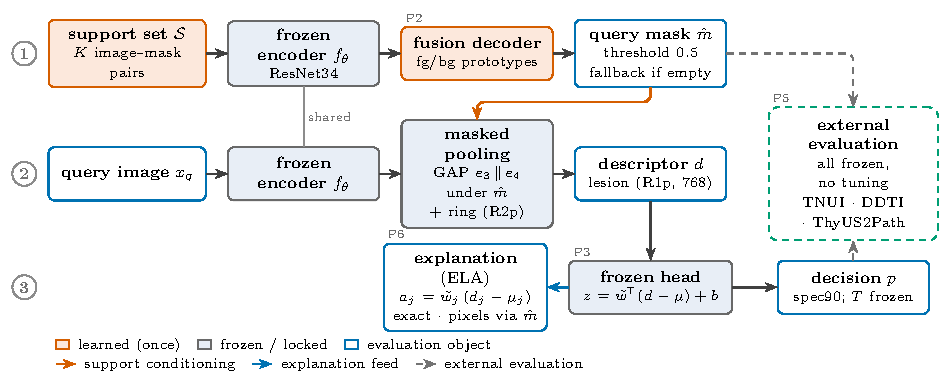
\includegraphics[width=0.95\linewidth]{fig1_standalone_preview.pdf}
\caption{\textbf{The LG-PM pipeline.} Top: a frozen support episode of
$K$ nested image--mask pairs from TN3K-train conditions the prototype
fusion decoder (trained once, Phase 2), which predicts the query mask
$\hat m$ at threshold $0.5$ with a whole-image fallback when the mask is
empty (rates in Supplementary Table~S17). Middle: the query
image passes the same frozen ResNet34 encoder (shared weights, vertical
link), and masked pooling averages its $e_3 \,|\, e_4$ features under
$\hat m$ (plus a $15$-px context ring in the R2p ablation), giving the
lesion descriptor $d$ (R1p, $768$-d; image-level R0 and lesion$+$ring
R2p $1536$-d variants: Supplementary Table~S4). Bottom: one linear head
trained once on TN5000-train, $z=\tilde w^{\top}(d-\mu)+b$, gives
$p=\sigma(z/T)$ with $T$ fitted on validation only and the operating
point frozen at $90\%$ specificity (raw--raw convention); the exact
linear attribution $a_j=\tilde w_j (d_j-\mu_j)$, $\sum_j a_j + c = z$,
is projected to pixels through $\hat m$ (Phase 6). Circled numerals mark
the three stages (1 support conditioning, 2 query encoding, 3 frozen
readout and attribution); the vermillion arrow is the support-conditioning
link, the blue arrow the explanation feed, and dashed arrows enter the
external-evaluation frame. P-badges mark the phase that produced each
object. Dashed frame: external evaluation on TNUI-2021, DDTI and
ThyUS2Path with every object frozen --- no target tuning, no target
calibration.}
\label{fig:pipeline}
\end{figure}


The architecture couples a shared encoder, a support-conditioned
segmentation module, a lesion--context descriptor module, and a family
of classification heads (Fig.~\ref{fig:pipeline}); the teacher's encoder
is an ImageNet-pretrained ResNet34 inside a U-Net-style decoder. The
working resolution is $384\times384$; the prototype module uses levels
$\{e_2, e_3, e_4\}$ (strides 8/16/32; 128/256/512 channels) and
descriptors pool $\{e_3, e_4\}$ (formal definitions: Supplementary
Section S3.1). Images are letterboxed; masks share the geometric
transform (nearest-neighbour) and are binarised at grey level
$\geq 127$, selected by visual audit against $>0$ and $\geq 250$
alternatives; inputs are ImageNet-normalised.

\subsubsection{Stage 1 optimisation (supervised reference)}

The Stage-1 reference is a ResNet34-encoder U-Net trained with the
Tversky-based objective below (optimiser, scheduler, augmentation, and
threshold-sweep listing: Supplementary Section S2.1). Each epoch selects
the better of raw and exponential-moving-average (EMA) weights by
validation Dice. The sigmoid operating threshold is tuned on the
internal validation split only and frozen before any test or external
evaluation; test-time augmentation (TTA) is reported alongside
single-view inference. The tuned threshold value is reported in
Results.

\subsubsection{Support-conditioned segmentation prototypes}

Each support mask is downsampled (nearest-neighbour) to the spatial
size of feature level $l$; the foreground prototype is the masked
average

\begin{equation}
  p_{f}^{l}
  = \frac{1}{Z_f^l}
    \sum_{i=1}^{K_m}\sum_{u}
    \bar{m}_{i}^{l}(u)F^l(x_i,u),
  \qquad
  Z_f^l=\sum_{i=1}^{K_m}\sum_u\bar{m}_{i}^{l}(u)+\epsilon,
  \label{eq:foreground_prototype}
\end{equation}

and the background prototype uses the complementary mask:

\begin{equation}
  p_{b}^{l}
  = \frac{1}{Z_b^l}
    \sum_{i=1}^{K_m}\sum_{u}
    (1-\bar{m}_{i}^{l}(u))F^l(x_i,u).
  \label{eq:background_prototype}
\end{equation}

Query pixel features are scored by the negative squared Euclidean
distance,

\begin{equation}
  s_{c}^{l}(x_q,u)
  =-\left\|F^l(x_q,u)-p_c^l\right\|_2^2,
  \qquad c\in\{f,b\},
  \label{eq:seg_similarity}
\end{equation}

score maps are bilinearly resized to the stride-8 grid ($48\times48$)
and stacked as $2L$ channels, and a lightweight convolutional decoder
$D_\phi$ ($2L\!\rightarrow\!32\!\rightarrow\!16\!\rightarrow\!1$)
produces the query mask:

\begin{equation}
  \hat m_q
  = \sigma\left(\,\mathrm{up}\!\left(
    D_\phi\bigl(\{s_f^l, s_b^l\}_{l}\bigr)\right)\right).
  \label{eq:query_mask}
\end{equation}

The \emph{direct} ablation replaces $D_\phi$ with the parameter-free sum
$\sum_l (s_f^l - s_b^l)$, isolating the learned fusion; Stage 2 freezes
the encoder (BatchNorm in inference mode) and trains only $D_\phi$. A
variance-weighted uncertainty extension is pre-specified (equations:
Supplementary Section S3.2) but was not executed: the point-prototype
model is the primary and only reported configuration.

\subsubsection{Lesion--context descriptor regimes}
\label{subsubsec:descriptor_regimes}

The representation module pools encoder features over five pre-specified
regions: for any binary mask $\Omega\in\{0,1\}^{H\times W}$ the
descriptor is the masked global average over levels
$l\in\{e_3, e_4\}$,

\begin{equation}
  z_{\Omega}(x)
  = \Big\Vert_{\,l\in\{e_3,e_4\}}
    \frac{\sum_u \tilde\Omega^{l}(u)\,F^{l}(x,u)}
         {\max\!\bigl(\sum_u \tilde\Omega^{l}(u),\,1\bigr)},
  \label{eq:masked_gap}
\end{equation}

computed per image (never across the batch).
Table~\ref{tab:regimes} defines the five regimes and the governing
conventions, all fixed before any evaluation.

\begin{table}[!ht]
\centering
\caption{\textbf{Lesion--context descriptor regimes (the five
pre-specified pooling regions).} Each is a masked global average over
encoder levels $\{e_3,e_4\}$ (Eq.~\eqref{eq:masked_gap}), computed per
image --- never across the batch --- and cached once per cohort in the
feature bank.}
\label{tab:regimes}
\begin{tabular}{@{}lp{72mm}p{34mm}@{}}
\toprule
Regime & Pooled region $\Omega$ (and fallbacks) & Role \\
\midrule
R0 & whole image (plain global average) & ungrounded reference \\
R1p & $\mathbf{1}[\hat m \geq 0.5]$, the binarised prediction from the
fixed support episode & deployable lesion grounding \\
R2p & lesion plus peri-lesional ring (elliptical dilation, radius
15\,px at $384^2$, minus the mask; empty ring falls back to the image
complement) & grounding $+$ context \\
R1g & oracle region (TN5000 expert box; TNUI-2021/DDTI ground-truth
mask) & oracle lesion; error-propagation pricing \\
R2g & oracle lesion plus its ring & grounding $+$ context, no
segmentation error \\
\bottomrule
\end{tabular}

{\footnotesize \emph{Governing conventions.} (1) \emph{Empty-mask
fallback}: fewer than 4 predicted pixels, and R1p/R2p pool the whole
image (identical to R0 for that case); the case is flagged and the
rate reported per cohort. (2) \emph{Oracle discipline}: oracle regions
appear only in the labelled oracle rows and the error-propagation
analysis, never in a deployable path. (3) \emph{Feature bank}: all five
regimes are computed once per cohort and cached with per-case quality
fields (Supplementary Section S2.6); the cache is the unit of reuse and
tolerance verification. (4) \emph{No learned fusion}: the ring contrast
(R1 versus R2) is reported explicitly as the context-utility
ablation.}
\end{table}

\subsubsection{Classification heads}
\label{subsubsec:classification_heads}

Three head families act on the cached descriptors; all supervision is
source-domain (TN5000 train) only.

\paragraph{Linear heads (primary).}
Each regime's descriptor is standardised with training-split statistics
and fitted with a logistic linear head under weighted binary
cross-entropy (training and selection protocol: Supplementary Section
S2.3). The only quantity that varies across regimes is \emph{what is
pooled}, so R0--R1p contrasts isolate grounding and R1p--R1g contrasts
isolate segmentation error.

{\sloppy
\paragraph{Class-prototype heads (annotation-efficiency analysis).}
Descriptors are L2-normalised, and per-class means over nested
per-class draws from the training split ($K_c \in
\{5,10,20,50,\allowbreak 200,\mathrm{all}\}$, 25 resamples per
finite budget, fixed seed) are scored by the cosine margin\par}

\begin{equation}
  s(x) = \cos\!\bigl(z(x),\mu_1\bigr) - \cos\!\bigl(z(x),\mu_0\bigr),
  \label{eq:cosine_margin}
\end{equation}

reported as mean $\pm$ standard deviation of test AUROC across draws;
in-domain only.

\paragraph{Whole-image ERM baseline (the fair comparator).}
The comparator is whole-image empirical risk minimisation (ERM): an
ImageNet-pretrained ResNet34 fine-tuned end-to-end on TN5000 (regimen:
Supplementary Section S2.4). This row must be strong --- it is the
conventional alternative a reviewer compares the grounded pipeline
against. A shrunk-covariance uncertainty scorer is a designated,
unreported extension.

\subsection{Training objectives}
\label{subsec:training_objectives}

The Stage-1 reference uses binary cross-entropy (BCE) plus a soft
Tversky term,

\begin{equation}
  \mathcal{L}_{\mathrm{seg}}^{(1)}
  =\mathcal{L}_{\mathrm{BCE}}+\mathcal{L}_{\mathrm{Tversky}},
  \qquad
  \mathcal{L}_{\mathrm{Tversky}}
  =1-\frac{\mathrm{TP}+\epsilon}
  {\mathrm{TP}+\alpha\,\mathrm{FP}+\beta\,\mathrm{FN}+\epsilon},
  \label{eq:stage1_loss}
\end{equation}

with $\alpha=0.3$, $\beta=0.7$, penalising false negatives on small,
fuzzy-boundary nodules. The Stage-2 decoder trains episodically with
query-pixel BCE plus a soft Dice term; the direct variant needs no
fitting. Classification heads minimise BCE with positive-class weight
$\omega = n_{\mathrm{neg}}/n_{\mathrm{pos}}$ from the source training
split. A boundary loss and an augmentation-consistency term were
considered and deferred.

\subsection{Training procedure}
\label{subsec:meta_training}

\textbf{Stage 1.} The ResNet34-UNet is trained on all TN3K
internal-training masks; the better of raw/EMA weights by validation
Dice is checkpointed; no external-domain image participates.
\textbf{Stage 2.} With the encoder frozen, the decoder alone is trained
on source episodes (nested supports, eight queries, light joint
augmentation applied consistently across images and masks), with early
stopping on mean query Dice over the validation episodes (regimen:
Supplementary Section S2.2); multi-source episodic training is a
designated extension.
\textbf{Stage 3.} The fixed support episode segments every TN5000 image
zero-shot; the five regimes are pooled and cached; the heads, budget
sweep, and ERM baseline are trained. This stage's checkpoint, cached
probabilities, and head parameters are the sole classification
artefacts permitted later.
\textbf{Stage 4.} On source validation only: a scalar temperature per
model (grid search; Supplementary Section S2.5), the decision threshold
(maximal sensitivity at specificity $\geq 0.90$ on raw validation
probabilities), the segmentation threshold, and the TTA configuration
--- all frozen before any test or external evaluation.
\textbf{Stage 5.} Frozen objects only cross domains, under
Section~\ref{subsec:external_classification_protocol}.

\subsubsection{Pre-registered joint partial-supervision phase (Phase 4)}
\label{subsec:phase4_preregistered}

Pre-registered before execution (full regimen: Supplementary Section
S4.1). A multi-task trunk (Stage-1 checkpoint, \emph{unfrozen}) is
fine-tuned on interleaved TN3K segmentation (BCE + Tversky) and TN5000
classification (weighted BCE) batches: \textbf{JOINT-g} classifies from
the trunk's \emph{own} predicted masks; \textbf{JOINT-img} pools the
whole image on the same trunk (grounding versus multi-tasking). The
head is first warmed on the frozen trunk, then jointly fine-tuned at
$10^{-5}$, an order of magnitude below the ERM regimen; checkpoint
selection maximises source validation AUROC \emph{subject to a
segmentation guard}, TN3K-validation Dice $\geq 0.8066$ (the
pre-registered non-collapse constant plus a $0.01$ margin), and the
test split never participates.

The guard exists because protocol v1 failed it: under a single-stage
joint fine-tune with AUROC-only selection, the freshly initialised
classification head's gradient rotated the shared encoder from the
first epoch --- saved-model TN3K-test Dice was 0.6686 against a gate of
0.7966 --- while a pristine-checkpoint control reproduced the locked
reference exactly, validating the harness. Should no joint epoch
satisfy the guard, the best-Dice state is retained for diagnosis and
the gate is allowed to fail: the joint phase is then reported as a
negative result rather than analysed. Both arms share identical
batch/augmentation streams (\texttt{set\_seed(42)} first) and differ
only in pooling region. The pre-declared in-domain family $G$ is headed
by G1, JOINT-g $-$ ERM AUROC (is the fine-tuning gap closed?); G2--G4
(frozen versus joint grounding; grounding versus multi-tasking;
operating-point contrast) are defined verbatim in Supplementary Section
S4.1. The joint model then enters the frozen external battery, its
thresholds and temperature fitted on its own TN5000 validation
probabilities only, under the manifest, non-collapse, and ERM-sanity
acceptance gates. A pre-registered uncertainty component reports
coverage-versus-malignant-FNR selective-prediction curves from
calibrated probabilities.

\subsubsection{Case-level external validation on ThyUS2Path (Phase 5)}
\label{subsec:phase5_preregistered}

Pre-registered before execution. ThyUS2Path contributes
histopathology-labelled cases from an acquisition network disjoint from
all source pools (two release batches, multiple images per case); the
question is whether the frozen pipeline and its pre-frozen operating
point survive a severe cohort-level shift under a pathology gold
standard. No metric cell runs before the audit gate, and no inferential
statement is unsealed before the licence (full A1--A5 mechanics:
Supplementary Section S4.2): per-batch label coverage must reach 95\%;
cases are scored by the unweighted mean of per-image calibrated
probabilities (first-image view as descriptive sensitivity analysis);
SHA-256 plus perceptual-hash screening against every support or
training pool excludes a \emph{whole} case on a single match; cohort
gates require 300 assembled cases and prevalence within $[0.20, 0.85]$;
and the operator attests label polarity against corpus documentation.
The family is computed under the seal but reported \textsc{withheld}
(descriptive statistics only) unless the gate passes computationally
\emph{and} attestation is complete; the amendment fixing the two-table
join, the case-mean primary unit, and whole-case exclusion was adopted
2026-08-22, strictly before any target-side forward pass.
Pre-registered family $J$ (case level; 5{,}000 paired bootstrap
resamples; Bonferroni $\alpha = 0.05/4 = 0.0125$; raw-raw convention;
nothing refitted) is headed by \textbf{J1}, sensitivity@spec90 R1p $-$
ERM with McNemar discordants on malignant cases --- the primary
external operating-point replication; J2--J4 are defined verbatim in
Supplementary Section S4.2. Oracle regimes are excluded by
pre-declaration (no lesion annotation).

\subsubsection{Pre-registered lesion-grounded explainability battery (Phase 6)}
\label{subsec:phase6_preregistered}

Pre-registered before execution; nothing is refitted and the only
backward passes compute activation gradients. For every linear head
(R0, R1p, R2p; JOINT-g, JOINT-img) the logit is exactly linear in the
pooled features, so per-pixel attribution is computed in closed form
within exactly the pooled regions (Exact Linear Attribution, ELA),
asserted to reproduce each head's logit to $<10^{-3}$; ERM uses
Grad-CAM at layer4 with Eigen-CAM and Score-CAM robustness rows, all
CAMs ReLU-ed and $\ell_1$-normalised. Four axes (full specifications
and perturbation recipes: Supplementary Section S4.3):
\emph{plausibility} --- explanation concentration in the TN5000 expert
box (localisation ratio: in-box explanation share over box-area share),
plus descriptive pointing games; \emph{faithfulness} --- deletion
(primary) and insertion curves against a per-image blur baseline and a
random-ordering control, the gap their trapezoidal area difference;
\emph{stability} --- Spearman correlation of clean and perturbed CAMs,
full pipeline recomputed; \emph{randomisation sanity} --- cascading
reinitialisation, self-gated at mean $\lvert\rho\rvert < 0.2$ at the
final stage (asserted). Cohorts: TN5000-test ($n{=}950$, 693 malignant;
expert boxes) and a seeded ThyUS2Path first-image panel ($n{=}600$,
from the licensed Phase-5 839-case manifest; label-free metrics,
independent of the Phase-5 licence). Pre-registered family $K$ (image
level; 5{,}000 paired bootstrap resamples; Bonferroni
$\alpha = 0.05/4 = 0.0125$; seed 42) is headed by \textbf{K1}, the
GT-localisation ratio R1p $-$ ERM on TN5000-test (primary
plausibility); K2--K4 are defined verbatim in Supplementary Section
S4.3.

\subsection{Baselines and ablation studies}
\label{subsec:baselines}

All baselines share the same cleaning, splits, preprocessing, episode
manifests, and seeds. Segmentation compares the full-data Stage-1
reference (TTA and single-view), parameter-free direct matching, the
proposed fusion-decoder model, and literature-style few-shot
architectures (PANet-, PFENet-, HSNet-like) under identical episodes,
subject to feasibility. The six pre-declared classification rows span
whole-image ERM, the R0/R1p/R2p grounding family, and the R1g/R2g
oracle rows, supplemented by the prototype budget sweep (annotation
efficiency) and the ring contrast (context utility). Further ablations:
ROI source (R0/R1g/R1p); ring on/off; nested budgets
$K_m\in\{1,5,10,20\}$ and $K_c$; zero-shot versus mask-shot; decoder
versus direct; frozen versus joint trunk; the deferred consistency
loss; the designated multi-source extension.

\subsection{Evaluation metrics}
\label{subsec:evaluation_metrics}

Dense segmentation evaluation reports per-case Dice,
intersection-over-union (IoU), sensitivity, precision, and the
95th-percentile Hausdorff distance (HD95; non-empty masks only;
definitions: Supplementary Section S3.3); episodic evaluation reports
per-episode Dice and IoU. Aggregate 95\% intervals use 2,000 bootstrap
replicates (image level for dense, episode means for episodic,
preserving episode pairing), and every external phase re-reports
segmentation quality control against the locked Phase-2 zero-shot
references before any classification table.

\subsubsection{Classification metrics and decision conventions}
\label{subsubsec:classification_metrics}

Reported metrics: AUROC; AUPRC; sensitivity at the validation-frozen
specificity-$0.90$ operating point; Brier score and expected
calibration error (ECE, 15 equal-width bins) around temperature
scaling; reliability curves for the headline rows. Four conventions
were fixed after the paired-analysis audit: (1) thresholds and
temperatures come from the source validation split only, frozen before
any test or external evaluation; (2) the raw-raw convention never mixes
raw-threshold binary decisions with calibrated probabilities (rank
metrics are convention-invariant); (3) confidence intervals are
case-level bootstrap, 2,000 resamples, percentile 2.5/97.5; (4)
externally, calibration metrics are descriptive only --- any deployment
interpretation requires local recalibration, stated rather than
performed.

\subsubsection{Selective prediction}

Referral scoring combines classification entropy and the probability
margin from calibrated probabilities (a Phase-4 pre-registered
component); risk--coverage curves report false-negative rate,
sensitivity, and error at prespecified coverage --- an assistive
mechanism, not an autonomous rule.

\subsection{External classification transfer protocol}
\label{subsec:external_classification_protocol}

This pre-registered protocol binds every external classification phase
and prevents silent refitting: the frozen objects --- encoder, fusion
decoder, fixed support episode (identifier-asserted), descriptor code,
head weights, thresholds, temperatures --- are byte-identical to the
source phase, and a battery of tolerance, sanity, quality-control, and
replication gates is checked before any external table, so that every
recomputed row must match its locked value within pre-set tolerances
and pooling-dependent analyses are \emph{withheld} rather than silently
recomputed (full gate specifications, tolerances, and pooling policy:
Supplementary Section S4.4). Exactly one pool is pre-declared
(TNUI-2021 test $+$ validation); later cohorts are individual families
with their own Bonferroni screens, and underpowered tests are labelled
as such, with direction-consistency reporting as the pre-declared
remedy.

\subsection{Statistical analysis}
\label{subsec:statistical_analysis}

The primary segmentation endpoint is external query Dice. The primary
classification endpoints are in-domain AUROC with the pre-declared
grounding and error-propagation contrasts and, externally, rank
discrimination (AUROC) plus the frozen specificity-$0.90$ operating
point --- the pooled operating point being the pre-declared
cross-cohort test. Intervals bootstrap at the most independent
available unit (image level in all current cohorts). Comparisons are
paired: both models are scored on identical case-level resamples with
two-sided sign-tail $p$-values,
$p = 2\min(\Pr[\Delta\leq0],\Pr[\Delta\geq0])$, and percentile 95\%
intervals; operating-point contrasts resample the malignant cases under
each model's frozen threshold; McNemar's $\chi^2$
(continuity-corrected) accompanies the in-domain operating-point
contrast. Resample counts: 5,000 in-domain, 2,000 external and pooled.
Multiplicity is controlled per pre-declared family by Bonferroni (0.05
divided by family size): family $T$ in-domain (six tests), families
$T_c/T_d/E/F/P$ externally (five each), family $G$ in the joint phase
(four). Effect sizes accompany $p$-values throughout; significance is
not interpreted as clinical usefulness without effect magnitude,
calibration, error type, and external-domain behaviour.

\subsection{Scope, reproducibility, and methodological boundaries}
\label{subsec:method_boundaries}

\emph{Explanation.}\label{subsec:explanation_method} The predicted mask
is the primary localisation output; class-specific explanations target
the reported classifier's decision score (the linear or joint head's
logit, or the cosine margin of Eq.~\eqref{eq:cosine_margin} for
prototype heads). The five analysis axes are executed as the
pre-registered Phase-6 battery
(Section~\ref{subsec:phase6_preregistered}), and ground-truth masks
serve explanation evaluation only unless an experiment is explicitly
designated mask-supervised.

\emph{Deployment outlook.}\label{subsec:edge_method} A deployment
pathway was designed and then deliberately descoped. The frozen
architecture admits a gradient-free mode in principle (supports encoded
once, prototype vectors cached), and a distilled mobile student with
FP32/FP16/INT8 exports would be benchmarked on size, memory, latency,
and degradation relative to the teacher. No student model, quantised
export, or latency measurement is reported; such results would be an
offline edge-feasibility simulation, not a clinical device validation.

\emph{Reproducibility.}\label{subsec:reproducibility} Clean manifests
are re-derived from raw files and hash-verified against the audit
manifests, and every reported table is generated from saved predictions,
not transcribed logs. The full artefact manifest --- dataset versions,
duplicate-drop lists, episode manifests, feature-bank caches, cached
probabilities, label parsers, the TNUI polarity record, locked
tolerance-reference tables, seeds, software versions, checkpoints ---
is listed in Supplementary Section S5, and Algorithm
S1\label{subsec:algorithm_summary} (Supplementary Section S6)
summarises the pipeline end to end. Target cohorts are never used for
architecture, threshold, calibration, or explainer selection.

\emph{Boundaries.} No ground-truth target mask enters ordinary
end-to-end inference: predicted-mask descriptors are the primary
condition; oracle regions appear only in the labelled oracle rows and
the error-propagation analysis. Labels are not silently harmonised
across provenance; the parsers, vote precedence, and TNUI polarity
record are released artefacts. External cohorts are never used for
fitting, tuning, thresholding, or calibration; pooling is limited to
the single pre-declared pool under the replication gate; the raw-raw
convention is fixed study-wide. The multi-source episodic extension,
the uncertainty-aware prototype, the shrunk-covariance scorer, and the
consistency loss are extension-level components; none is claimed in the
primary pipeline.

%======================================================================
% sec16_results.tex - COMPRESSED main-text Results (16-page split,
% operator commission 2026-08-23, stage 2 of 5).
% Kept tables: test_families, cohorts, phase2, evidence (verbatim) and
% the four pre-registered family tables trimmed to primary rows (rows
% relocated verbatim to sm_results.tex Tables S5/S22). Per-cohort and
% operational tables -> Supplementary Tables S1-S22; Figures S1-S2.
% No number altered; negatives/nulls/reversals/failed gates remain here.
%======================================================================

\section{Results}\label{sec:results}

Ten pre-registered test families organise the inferential results.
Table~\ref{tab:test_families} maps each family's letter to its cohort,
the research question it answers, and its phase; the prose uses short
descriptive names, with letters retained in tables for precision.
Per-cohort and operational tables are consolidated in the Supplementary
Information (Tables S1--S22); the main text leads each phase with its
consolidated or family-level table.

\begin{table}[!ht]
\centering\small
\setlength{\tabcolsep}{4pt}
\caption{Pre-registered test families: letter, cohort, motivating
research question (Section~\ref{sec:research_questions}), and phase.
Test rosters and per-family Bonferroni screens are fixed in
Section~\ref{subsec:statistical_analysis} and the phase protocols. The
class-prototype label-budget sweep (Phase 3) and selective prediction
(Phase 4) are pre-registered components reported outside the lettered
families.}
\label{tab:test_families}
\begin{tabular}{lp{3.3cm}p{3.1cm}ll}
\toprule
Family & Name used in prose & Cohort (unit) & RQ & Phase \\
\midrule
T  & in-domain TN5000 family & TN5000 test (image) & RQ3, RQ4, RQ6 & 3b \\
Tc & TNUI-test family & TNUI-2021 test (image) & RQ2, RQ3 & 3c \\
Td & TNUI-val family & TNUI-2021 val (image) & RQ2, RQ3 & 3d \\
P  & TNUI-pool family & TNUI test+val pool (image) & RQ2, RQ3 & 3d \\
E  & DDTI family & DDTI (image) & RQ2 & 3e \\
F  & TNUI-train probe & TNUI-2021 train (image) & RQ2 & 3e \\
G  & joint in-domain family & TN5000 test (image) & RQ5 & 4 \\
H  & joint pooled family & TNUI test+val pool (image) & RQ5 & 4 \\
J  & ThyUS2Path case family & ThyUS2Path (case) & RQ2, RQ3 & 5 \\
K  & explanations family & TN5000 + ThyUS-600 (image) & RQ8 & 6 \\
\bottomrule
\end{tabular}
\end{table}

\subsection{Cohorts, audits, and frozen operating conventions}
\label{subsec:res_cohorts}

Table~\ref{tab:cohorts} summarises the audited cohorts entering the
classification battery; deduplication, cross-dataset hashing, and the
official split files were applied as in
Section~\ref{sec:methodology_revised}. The TN5000 manifest re-derived
byte-identically in every phase (3, 3b--3e), and the Phase-3d/3e
replication gates reported zero drift on every replicated cell
(\textsc{pooled\_ok}). Segmentation quality control preceded any
classification table on every external cohort, against the Phase-2
zero-shot references (TNUI 0.7079, DDTI 0.6782 at $K{=}20$; per-cohort
QC rows: Supplementary Table~S1). Empty-mask fallback was rare
in-domain (1.1\% val / 1.2\% test, Table~\ref{tab:cohorts}).

\begin{table}[!ht]
\centering\scriptsize
\setlength{\tabcolsep}{4pt}
\caption{Classification cohorts after audit (locked). $n$ = usable cases;
prev.\ = malignant prevalence. TN5000 is the source domain; TNUI-2021 splits
and DDTI are zero-shot external cohorts.}
\label{tab:cohorts}
\begin{tabular}{llrrl}
\toprule
Cohort & Role & $n$ & malignant (prev.) & Notes \\
\midrule
TN5000 train & source fit & 3448 & 2430 (0.705) & clinical split file train.txt \\
TN5000 val   & thresholds/temperature & 476 & 360 (0.756) & val.txt \\
TN5000 test  & in-domain evaluation & 950 & 693 (0.729) & test.txt \\
TNUI-2021 test  & external (3c) & 139 & 134 (0.964) & 0 cross-dups vs TN5000 \\
TNUI-2021 val   & external (3d) & 274 & 258 (0.942) & 1 val--test cross-dup excluded \\
TNUI-2021 train & external probe (3e) & 966 & 915 (0.947) & pooled policy n/a \\
DDTI (XML-labelled) & independent external (3e) & 189 & 145 (0.767) & 1 within-dup dropped \\
\bottomrule
\end{tabular}
\end{table}

\subsection{Supervised segmentation reference and external gap (Phase 1)}
\label{subsec:res_phase1}

The full-data ResNet34-UNet reference (single seed, validation-only
threshold 0.60, test-time augmentation, TTA) defines the
annotation-expensive ceiling: the in-domain TTA Dice sits within the
published TN3K band, and the external rows quantify the domain-shift
cost before any few-shot machinery (full table: Supplementary
Table~S2). TTA effects are small and sign-mixed --- the largest shift
is $+1.11$ Dice points on TNUI-all, and DDTI moves slightly in the
opposite direction --- and DDTI is visibly the harder masked cohort
(sensitivity 0.83, median HD95 roughly doubled), consistent with its
lower zero-shot prototype scores below.

\subsection{Few-shot support-conditioned segmentation (Phase 2)}
\label{subsec:res_phase2}

\begin{figure}[H]
\centering
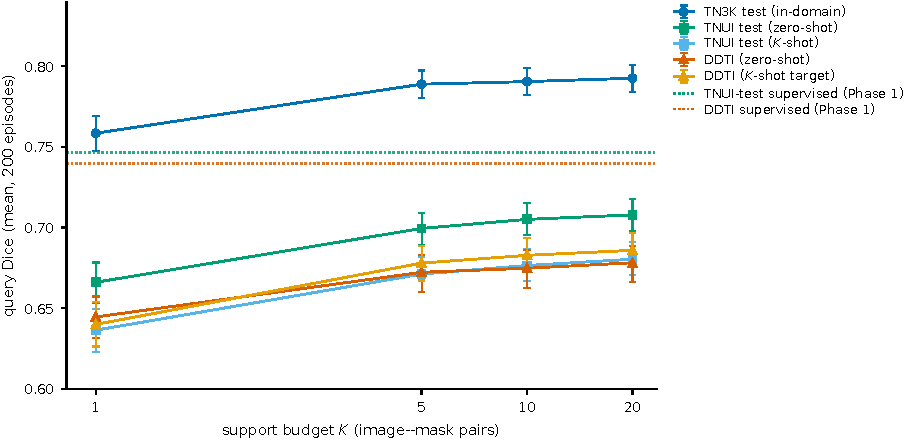
\includegraphics[width=0.95\linewidth]{fig2_budget_dice.pdf}
\caption{\textbf{Few-shot segmentation saturates early and transfers
without target annotation.} Query Dice (fusion decoder) versus support
budget $K$ with nested episodes (200 episodes per cell, 1{,}600 query
predictions; error bars: episode-blocked bootstrap 95\% CIs). Dotted
lines: the fully supervised Phase-1 external references. Zero-shot
source-support transfer lands within 3.9 (TNUI-2021) and 6.1 (DDTI)
Dice points of the supervised external reference at $K{=}20$ and
already captures 98.6--99.5\% of it at $K{=}5$; the parameter-free
direct-matching variant (Supplementary Table~S3) is 3.2--20.9
points lower in every cell.}
\label{fig:budget}
\end{figure}


Episodic evaluation (200 episodes per condition, $Q_m{=}8$, nested
budgets) yields three findings (Table~\ref{tab:phase2}). (i) The
learned fusion decoder outperforms parameter-free direct matching in
all 20 condition--budget cells, by $+3.2$ to $+20.9$ Dice points (full
rows: Supplementary Table~S3). (ii) The annotation budget saturates
early: $K{=}5$ already delivers 98.6--99.5\% of the $K{=}20$ score in
all conditions (Fig.~\ref{fig:budget}). (iii) Zero-shot transfer with
source supports lands within $3.9$ Dice points of the supervised
external reference on TNUI (0.7079 vs 0.7464) and within $6.1$ on DDTI
(0.6782 vs 0.7396), while using \emph{zero} target annotations. Best
validation episodic Dice 0.7776 (epoch 13; early stop 21; 37.7 min).
The support-domain bias observed on TNUI (target supports underperform
source supports) is reported as a limitation and motivates the
joint-resourcing question of Phase 4.

\begin{table}[!ht]
\centering\scriptsize
\caption{Phase-2 query Dice by support budget $K_m$ (fusion decoder; locked).
200 episodes per cell ($Q_m{=}8$; 1,600 query predictions), episode-blocked
bootstrap 95\% CIs in parentheses. Last column: decoder advantage over
parameter-free direct matching at $K{=}20$ (full direct rows in
Supplementary Table~S3).}
\label{tab:phase2}
\lgShrink{%
\begin{tabular}{lccccc}
\toprule
Condition & $K{=}1$ & $K{=}5$ & $K{=}10$ & $K{=}20$ & $\Delta$direct (K20, pts) \\
\midrule
TN3K test (in-domain)  & 0.7585 (0.7477--0.7694) & 0.7889 (0.7806--0.7974) & 0.7905 (0.7822--0.7987) & 0.7926 (0.7843--0.8008) & +11.7 \\
TNUI test (zero-shot)  & 0.6661 (0.6534--0.6784) & 0.6995 (0.6894--0.7092) & 0.7051 (0.6952--0.7152) & 0.7079 (0.6979--0.7178) & +20.9 \\
TNUI test ($K$-shot)   & 0.6364 (0.6227--0.6498) & 0.6712 (0.6603--0.6818) & 0.6765 (0.6668--0.6866) & 0.6804 (0.6705--0.6909) & +5.3 \\
DDTI (zero-shot)       & 0.6446 (0.6317--0.6573) & 0.6723 (0.6603--0.6832) & 0.6748 (0.6627--0.6859) & 0.6782 (0.6665--0.6888) & +11.0 \\
DDTI ($K$-shot target) & 0.6400 (0.6263--0.6537) & 0.6780 (0.6672--0.6887) & 0.6828 (0.6727--0.6933) & 0.6859 (0.6760--0.6964) & +3.3 \\
\bottomrule
\end{tabular}%
}
\end{table}

\subsection{In-domain classification with frozen descriptors (Phases 3 and 3b)}
\label{subsec:res_phase3}

All heads share the frozen Phase-1 encoder, the fixed $K_m{=}20$ TN3K
support episode, and identical training regimens; thresholds
(specificity $\geq 0.90$ on raw validation probabilities) and
temperatures are frozen from validation only. In-domain level rows
(AUROC: ERM 0.9401, R1p 0.8902, oracle R1g 0.9105) and the per-model
frozen operating points appear in Supplementary Tables~S4 and~S6; the
pre-registered paired battery is Table~\ref{tab:phase3b}. Lesion
grounding beats the identical frozen whole-image head (T1: $+0.0368$,
$p{=}0.0004$), and fine-tuning remains the in-domain rank ceiling (T2:
$+0.0498$, $p{<}0.0004$). The secondary contrasts (relocated rows:
Supplementary Table~S5) price error propagation directly (T3:
$+0.0202$, $p{=}0.0048$; sens@spec90 analogue T6: $+0.0982$,
$p{<}0.0004$) and return two negative or null findings that we report
as such: the context ring adds nothing (T4: $+0.0074$, $p{=}0.1388$;
hypothesis H6 is null), and ERM dominates the in-domain operating
point (T5: $-0.0749$, $p{<}0.0004$).

Two calibration readings are worth flagging in-domain: fitted
temperatures are $T<1$ for every frozen-descriptor head (mildly
\emph{under}-confident logits) but $T=1.969$ for ERM
(over-confident); and ERM is the best-calibrated model in-domain
(Brier 0.0878, ECE 0.0634). Neither property survives the external
shift, as the external battery shows below.

Error propagation is diffuse rather than confidence-localised
(quartile table: Supplementary Table~S7): the oracle-minus-predicted
AUROC gap is modest in the lowest-confidence quartiles, vanishes in
Q3, and is descriptively largest in the \emph{highest}-confidence
quartile ($+0.0589$), the mean gap ($\approx$0.022) closely matching
the global T3 contrast. Segmentation error therefore imposes a diffuse
$\approx$2-point tax on grounded features, and there is no
confidence-gated ``safe subgroup'' in which predicted masks are
output-equivalent to oracle boxes.

The class-prototype label-budget sweep ($K$ per class
$\in \{5,10,20,50,200,\mathrm{all}\}$, 25 draws; Supplementary
Table~S8) carries the classification-side annotation-efficiency claim:
grounding dominates the identical whole-image budget at every $K$
($+0.046$ to $+0.096$ AUROC); R1p saturates by $K{=}50$ (0.6383 versus
0.6379 full-budget) and stays within 0.013--0.029 of the oracle, while
R0 has not saturated even at $K{=}200$; and the ring is
null-or-negative throughout (R2p $\leq$ R1p, R2g $\leq$ R1g at every
$K$), corroborating the T4 null under a different head family.
Absolute levels sit far below the linear heads (0.59--0.66 vs
0.85--0.91), as expected for a cosine prototype rule on frozen
descriptors; the linear head remains the pre-declared primary
classifier.

\begin{table}[!ht]
\centering\small
\caption{Phase-3b paired tests (locked; 5000 paired bootstrap resamples,
Bonferroni $\alpha = 0.0083$; McNemar $\chi^2$ on discordant malignant
cases). $\Delta$ = A$-$B. Empirical $p$-values are floored by the resample
count: reports of $p{<}0.0004$ denote zero zero-crossings in 5000 resamples.}
\label{tab:phase3b}
\begin{tabular}{clllccl}
\toprule
Test & Contrast & Metric & $\Delta$ (95\% CI) & $p$ & Sig. & Interpretation \\
\midrule
T1 & R1p $-$ R0  & AUROC & +0.0368 (0.0161, 0.0589) & 0.0004 & YES & grounding $>$ image \\
T2 & ERM $-$ R1p & AUROC & +0.0498 (0.0308, 0.0691) & $<$0.0004 & YES & fine-tune rank ceiling \\
\midrule
\end{tabular}

{\footnotesize Secondary contrasts T3--T6 (with the T5 McNemar pair), relocated row-for-row: Supplementary Table~S5.}
\end{table}

\subsection{External classification battery (Phases 3c, 3d, 3e)}
\label{subsec:res_external}

All external rows are computed with the frozen source objects;
thresholds and temperatures come from TN5000 validation only, and no
target case informed any decision. Per-cohort families are
Bonferroni-screened at $\alpha = 0.01$; the single pre-declared pool is
TNUI test+val with its own family. Table~\ref{tab:evidence}
consolidates the matrix: all cohorts, all six models.

\paragraph{TNUI-2021 test (Phase 3c).}
$n{=}139$ (134 malignant). Grounding degrades least: the AUROC shift
drop shrinks monotonically with lesion-centring strength, from ERM's
0.423 down to R2g's 0.052. The fine-tuned ERM operating point does not
transfer (T5c: $-0.157$, $p{=}0.0028$) --- an inversion of the
in-domain T5 ($+0.075$ ERM advantage) --- and ERM sits significantly below the true-mask oracle
(T4c: $-0.3170$, $p{=}0.0004$); T1c--T3c are power-limited (5 benign
cases). Rows: Supplementary Table~S9.

\paragraph{Second cohort and pooled test (Phase 3d).}
TNUI-2021 val ($n{=}274$, 16 benign) discriminates poorly for
\emph{every} model including true-mask oracles (0.577--0.624),
revising the friendly-cohort reading of 3c; the replication gate
passed with zero drift. The pre-declared TNUI-pool family found the
grounded heads' operating-point advantage over ERM replicated and
significant (P5: $-0.120$, CI $-0.181..-0.061$, $p{<}0.0004$); the
rank-transfer flip of 3c did not replicate (P2 null). Rows:
Supplementary Table~S10.

\paragraph{Independent-institution counterexample and heterogeneity
probe (Phase 3e).}
DDTI ($n{=}189$, 44 benign) sits at chance for \emph{all} models ---
including below-0.5 true-mask oracles (0.414--0.422) --- and the
operating point inverts: ERM wins (E5: $+0.1456$, $p{=}0.0012$).
TNUI-train ($n{=}966$) behaves like val ($\approx$0.55--0.65),
confirming 3c's test split as the friendly cohort; burned-in DDTI
acquisition annotations are a documented confound (qualitative grid).
Rows: Supplementary Table~S11.

\paragraph{External verdict (as locked).}
(i) In-domain ranks are fixed (Table~\ref{tab:evidence}, first row). (ii)
External rank discrimination is cohort-dominated: identical frozen
rules swing the true-mask oracle over 0.42--0.85
(Table~\ref{tab:evidence}). (iii) The grounded operating point
(Supplementary Figure~S1) transfers across the TNUI institutional
family (test $p{=}0.0028$; train and pooled $p{<}0.0004$; val in
direction) and \emph{reverses} on the independent DDTI cohort
($p{=}0.0012$): an institutional-family transfer claim with a
documented counterexample. (iv) Calibration does not survive the
prevalence shift in any model (external ECE 0.25--0.42); rank metrics
therefore remain primary externally, and deployment claims require
local recalibration.

\begin{table}[!ht]
\centering\small
\caption{Cross-cohort evidence matrix (AUROC; locked rows). Sign consistency of
R1p$-$ERM: AUROC $+,-,+,+$; sens@spec90 $+,+,+,-$ across TNUI test/val/train
and DDTI. Oracle (R1g) AUROC externally: 0.834/0.613/0.646/0.422.}
\label{tab:evidence}
\begin{tabular}{lcccccc}
\toprule
Cohort & ERM & R0 & R1p & R2p & R1g (oracle) & R2g (oracle) \\
\midrule
TN5000 test (in-domain) & 0.9401 & 0.8534 & 0.8902 & 0.8829 & 0.9105 & 0.9029 \\
TNUI test   & 0.5172 & 0.5791 & 0.7119 & 0.6776 & 0.8343 & 0.8507 \\
TNUI val    & 0.6237 & 0.5901 & 0.5775 & 0.6008 & 0.6126 & 0.5770 \\
TNUI train  & 0.5936 & 0.5472 & 0.6316 & 0.6441 & 0.6459 & 0.6078 \\
DDTI        & 0.4746 & 0.5116 & 0.4967 & 0.5017 & 0.4216 & 0.4143 \\
\bottomrule
\end{tabular}
\end{table}

\subsection{Joint partial-supervision fine-tuning (Phase 4)}
\label{subsec:res_phase4}

Phase 4 asked whether the segmentation pathway can be kept intact while
a classification head is fine-tuned into the shared trunk, and whether
doing so closes the in-domain fine-tuning gap (T2). Protocol v1
(single-stage joint fine-tune at $10^{-4}$, AUROC-only selection)
failed the pre-registered segmentation non-collapse gate outright
(TN3K-test Dice 0.6686 against a gate of 0.7966; triage showed the
fresh head's gradients rotating the shared encoder from the first
epoch). Protocol v2 --- trunk-frozen head warmup, a low-rate
($10^{-5}$) joint phase, and seg-guarded checkpoint selection on the
validation split only --- passed both non-collapse gates (JOINT-g
0.8258, JOINT-img 0.8165 against the same 0.7966 gate), with frozen-row
integrity exact (ERM 0.9401, R1p 0.8902).

The joint in-domain family G (Table~\ref{tab:phase4_families}; level
rows: Supplementary Table~S12) answers the motivating question in the
negative, and we report it as such: joint training did \emph{not} close
T2 --- it widened it (G1: $-0.0703$, CI $-0.0927..-0.0486$,
$p{<}0.0004$). JOINT-g also sits \emph{below} the frozen grounded head
it was meant to surpass (G2: $-0.0205$, CI $-0.0365..-0.0045$;
$p{=}0.0124$, clearing the family bar by $10^{-4}$ --- significant but
fragile). The one large positive is mechanistic: under identical
multi-task conditions the grounded head beats the whole-image head by
14.9 points (G3: $+0.1489$, CI 0.1136..0.1848) --- the grounding
advantage survives joint optimisation; it is not an artefact of
freezing. At the pre-frozen operating point the joint model loses
outright (G4: $-0.2376$ CI $-0.2785..-0.1962$; McNemar 41 vs 206 on
test positives, $\chi^2{=}108.89$; G2--G4 rows: Supplementary
Table~S5). JOINT-g had not saturated at the pre-registered 15-epoch cap
(validation AUROC was still improving; the cap was not extended), so
family-G magnitudes are conservative.

The pair of runs documents a precise dilemma: closing the T2 gap
requires the task-specific representational reorganisation ERM performs
from scratch, and any such reorganisation is precisely what a
segmentation non-collapse constraint forbids. v1 unknowingly chose one
horn (fine-tuning performance without an intact segmenter); v2 proves
the other (an intact segmenter without the fine-tuning premium).

The external family H completes the picture
(Table~\ref{tab:phase4_families}; level rows: Supplementary Table~S13).
The primary external test is nominal only: on the single locked
TNUI test+val pool JOINT-g exceeds ERM's sensitivity at the frozen
operating point by 6.6 points (H1: $+0.0661$, 95\% CI 0.005..0.128,
$p{=}0.033$, beyond the family bar; McNemar 86 vs 60). The rank test
is a flat null (H3: $-0.011$, $p{=}0.858$; secondary rows:
Supplementary Table~S5), and H2 is significant: joint grounding
transfers its operating point \emph{worse} than the frozen R1p by 5.3
points of pooled sensitivity (H2: $-0.0534$, CI $-0.097..-0.010$,
$p{=}0.011$). The
pooled operating-point ordering, R1p $\approx 0.666$ $>$ JOINT-g
$\approx 0.612$ $>$ ERM $\approx 0.546$, is the distilled Phase-4
verdict. The joint segmenter travels adequately (external Dice
0.674--0.765, empty-mask $\leq 0.3\%$), so the deficit lives in
classification head-room, not mask collapse. Every Phase-4 strand
converges on the same operational choice: \emph{the frozen-descriptor
R1p pipeline is the primary LG-PM model}.

The pre-registered selective-prediction component (Supplementary
Table~S14; Supplementary Figure~S2) shows calibrated-margin abstention
biting at the frozen operating point without any refitting: retaining
the most-confident 70\% of TN5000-test cases lifts JOINT-g's
sensitivity at spec90 from 0.564 to 0.840, and at 50\% coverage the
curve reaches 0.874 in-domain and 0.897 on the external TNUI pool. The
effect is referral-shaped, not accuracy-shaped: approximately
86--87\% of the frozen point's malignant misses sit inside the
abstained lower-confidence half on both panels (261 of 302 misses
in-domain; 132 of 152 on pooled TNUI). No threshold or temperature was
re-estimated for these numbers (raw-raw; the validation-fitted
$T{=}0.523$ supplies only the confidence margin).

\begin{table}[!ht]
\centering\small
\caption{Phase-4 pre-registered families. G (in-domain TN5000 test; 5,000
paired bootstrap resamples, Bonferroni $\alpha{=}0.0125$): \emph{locked}.
H (pooled TNUI test+val, $n{=}413$, 392 positives, 2,000 resamples,
$\alpha{=}0.0167$): \emph{locked}.
$\Delta$ = A$-$B; empirical $p$ floored as $p{<}0.0004$
(zero zero-crossings in 5,000 resamples). H1's 95\% CI excludes zero while
$p{=}0.033$ exceeds the family bar (the $\approx$98.3\% CI includes zero):
reported as nominal.}
\label{tab:phase4_families}
\lgShrink{%
\begin{tabular}{clllccl}
\toprule
Test & Contrast & Metric & $\Delta$ (95\% CI) & $p$ & Sig. & Question \\
\midrule
G1 & JOINT-g $-$ ERM & AUROC & $-$0.0703 ($-$0.0927, $-$0.0486) & $<$0.0004 & YES & is the T2 fine-tune gap closed? --- \textbf{No: widened} \\
\midrule
H1 & JOINT-g $-$ ERM & sens@spec90 (pooled) & +0.0661 (0.0051, 0.1276) & 0.033 & no & PRIMARY external op.\ point --- nominal only \\
\multicolumn{7}{l}{McNemar (H1, pooled positives $n{=}392$): JOINT-g-right/ERM-wrong 86 vs ERM-right/JOINT-g-wrong 60,}\\
\multicolumn{7}{l}{$\chi^2 = 4.28$ (nominal $p \approx 0.039$) --- direction consistent, family bar not cleared.}\\
\bottomrule
\end{tabular}%
}

{\footnotesize Secondary contrasts G2--G4 (with the G4 McNemar pair) and H2--H3, relocated row-for-row: Supplementary Table~S5.}
\end{table}

\subsection{Case-level external validation on ThyUS2Path (Phase 5)}
\label{subsec:res_phase5}

Phase 5 carried the frozen pipeline onto ThyUS2Path, a
histopathology-labelled cohort from an acquisition network disjoint
from all source pools, under the audit-gated licence protocol
(Section~\ref{subsec:phase5_preregistered}) --- the study's central
external-validation demand: a second, pathology-verified institution,
evaluated at case level. The audit passed end to end: label coverage
was complete for Batch 1 (6{,}005/6{,}005) and near-complete for Batch
2 (2{,}495/2{,}503), giving an overall parse rate of 0.9991
(8{,}500/8{,}508); the surviving join matched the corpus's own image
map exactly (5{,}893/5{,}893 Batch-1 stems). Assembly gave 842
cases (601 + 241), and conservative whole-case near-duplicate
screening excluded three, leaving 839 cases and 8{,}465 images
(598 + 241), of which 522 are malignant
(prevalence 0.622, inside the $[0.20, 0.85]$ gate). Frozen-row
integrity held exactly (ERM re-hit 0.9401; the retrained R1p head
reproduced 0.8889 against the locked 0.8902, within the 0.002
integrity tolerance; both
JOINT arms matched to $\leq 10^{-6}$, temperatures 0.523/0.200), and
segmentation QC was healthy (empty masks on 10.9\% of images,
926/8{,}465; JOINT-g decoder 3.5\% (293/8{,}465)). Mean predicted
nodule areas were 4.1\% and 5.9\% of the frame respectively. The
cohort ships without lesion
annotation, so no external Dice is computable and the oracle regimes
are excluded as pre-declared. Label polarity was operator-attested on
the seeded audit grid, whereupon the inference licence was granted; the
licence upgrade unsealed the significance column and altered no number.

Ranking collapses universally (per-model rows: Supplementary
Table~S15; shift matrix: Supplementary Table~S16): all six models land
between AUROC 0.478 and 0.548 on the case unit, only ERM's interval
clearing 0.5 --- by eight thousandths. AUPRC spans 0.608--0.666
against the 0.622 prevalence, and shift drops from source are
0.31--0.39 AUROC for every linear head and 0.39 for
ERM (drop 0.3921, the largest); even JOINT-img, modest in-domain (0.7207), loses 0.24, and
the first-list-image view shows the same pattern (0.481--0.533;
Supplementary Table~S17). Two observations place the collapse at
cohort level rather than in the LG-PM machinery: it afflicts ERM ---
a pure whole-image classifier with no segmentation in the loop --- at
least as severely as any descriptor head, and it persists when case
aggregation is bypassed entirely. Calibration does not travel either:
source-fitted temperatures \emph{worsen} external ECE for five of six
models (post-calibration ECE 0.26--0.31; only ERM improves, 0.2813
$\to$ 0.2145), and Brier scores (0.29--0.35) sit far above the source
regime.

The pre-registered case family J replicates the operating-point story
at full strength (Table~\ref{tab:phase5_familyj}). At the frozen
specificity-$\geq$0.90 thresholds, the grounded descriptor retains
15.9\% case-level sensitivity where the fine-tuned ERM retains 1.3\%
(J1: $+0.1457$, 95\% CI 0.1149..0.1782, $p{<}0.0004$; McNemar 77 vs 1,
$\chi^2 = 72.12$, $p < 10^{-4}$). In integers: of the 83 malignant
cases R1p catches at the frozen point, ERM misses 77; of the 7 ERM
catches, R1p misses 1 --- an eleven-fold relative advantage, and the
external case-level replication of the internal operating-point result.
Frozen-over-joint transfer replicates with larger magnitude (J3:
$-0.0978$, CI $-0.1264..-0.0709$, $p{<}0.0004$), and the case-level
operating-point ordering, R1p (0.1590) $>$ JOINT-g (0.0613) $>$ ERM
(0.0134), mirrors the pooled Phase-4 ordering (0.666 $>$ 0.612 $>$
0.546) across an entirely disjoint cohort. The rank contrasts are null
at the family bar (J2 $p{=}0.0436$; J4 $p{=}0.1104$; rows:
Supplementary Table~S5). The honest reading is twofold: absolute
performance on ThyUS2Path is far from diagnostic grade for
\emph{every} model --- 15.9\% sensitivity at 90\% specificity is a
comparative, not a clinical, statement --- and the cohort functions as
a stress test of what survives a severe acquisition and case-mix
shift; what survives is precisely the lesion grounding.

\begin{table}[!ht]
\centering\small
\caption{Phase-5 pre-registered family J (ThyUS2Path case level,
$n{=}839$, 522 malignant; 5{,}000 paired case-bootstrap resamples;
Bonferroni $\alpha{=}0.0125$): \emph{locked}. $\Delta$ = A$-$B; empirical
$p$ floored as $p{<}0.0004$ (zero zero-crossings in 5{,}000 resamples).
Computed under the sealed audit-gate discipline and unsealed only after
A1--A4 passed and the operator attested label polarity (A5); the licence
upgrade altered no number in this table.}
\label{tab:phase5_familyj}
\lgShrink{%
\begin{tabular}{clllccl}
\toprule
Test & Contrast & Metric & $\Delta$ (95\% CI) & $p$ & Sig. & Question \\
\midrule
J1 & R1p $-$ ERM      & sens@spec90 & +0.1457 (0.1149, 0.1782)     & $<$0.0004 & YES & PRIMARY external op.\ point --- \textbf{replicated} \\
\multicolumn{7}{l}{McNemar (J1, malignant cases $n{=}522$): R1p-right/ERM-wrong 77 vs ERM-right/R1p-wrong 1,}\\
\multicolumn{7}{l}{$\chi^2 = 72.12$ ($p < 10^{-4}$) --- 77:1 discordants in favour of the grounded head at the frozen point.}\\
\bottomrule
\end{tabular}%
}

{\footnotesize Secondary contrasts J2--J4, relocated row-for-row: Supplementary Table~S5.}
\end{table}

\subsection{Lesion-grounded explainability battery (Phase 6)}
\label{subsec:res_phase6}

\begin{figure}[H]
\centering
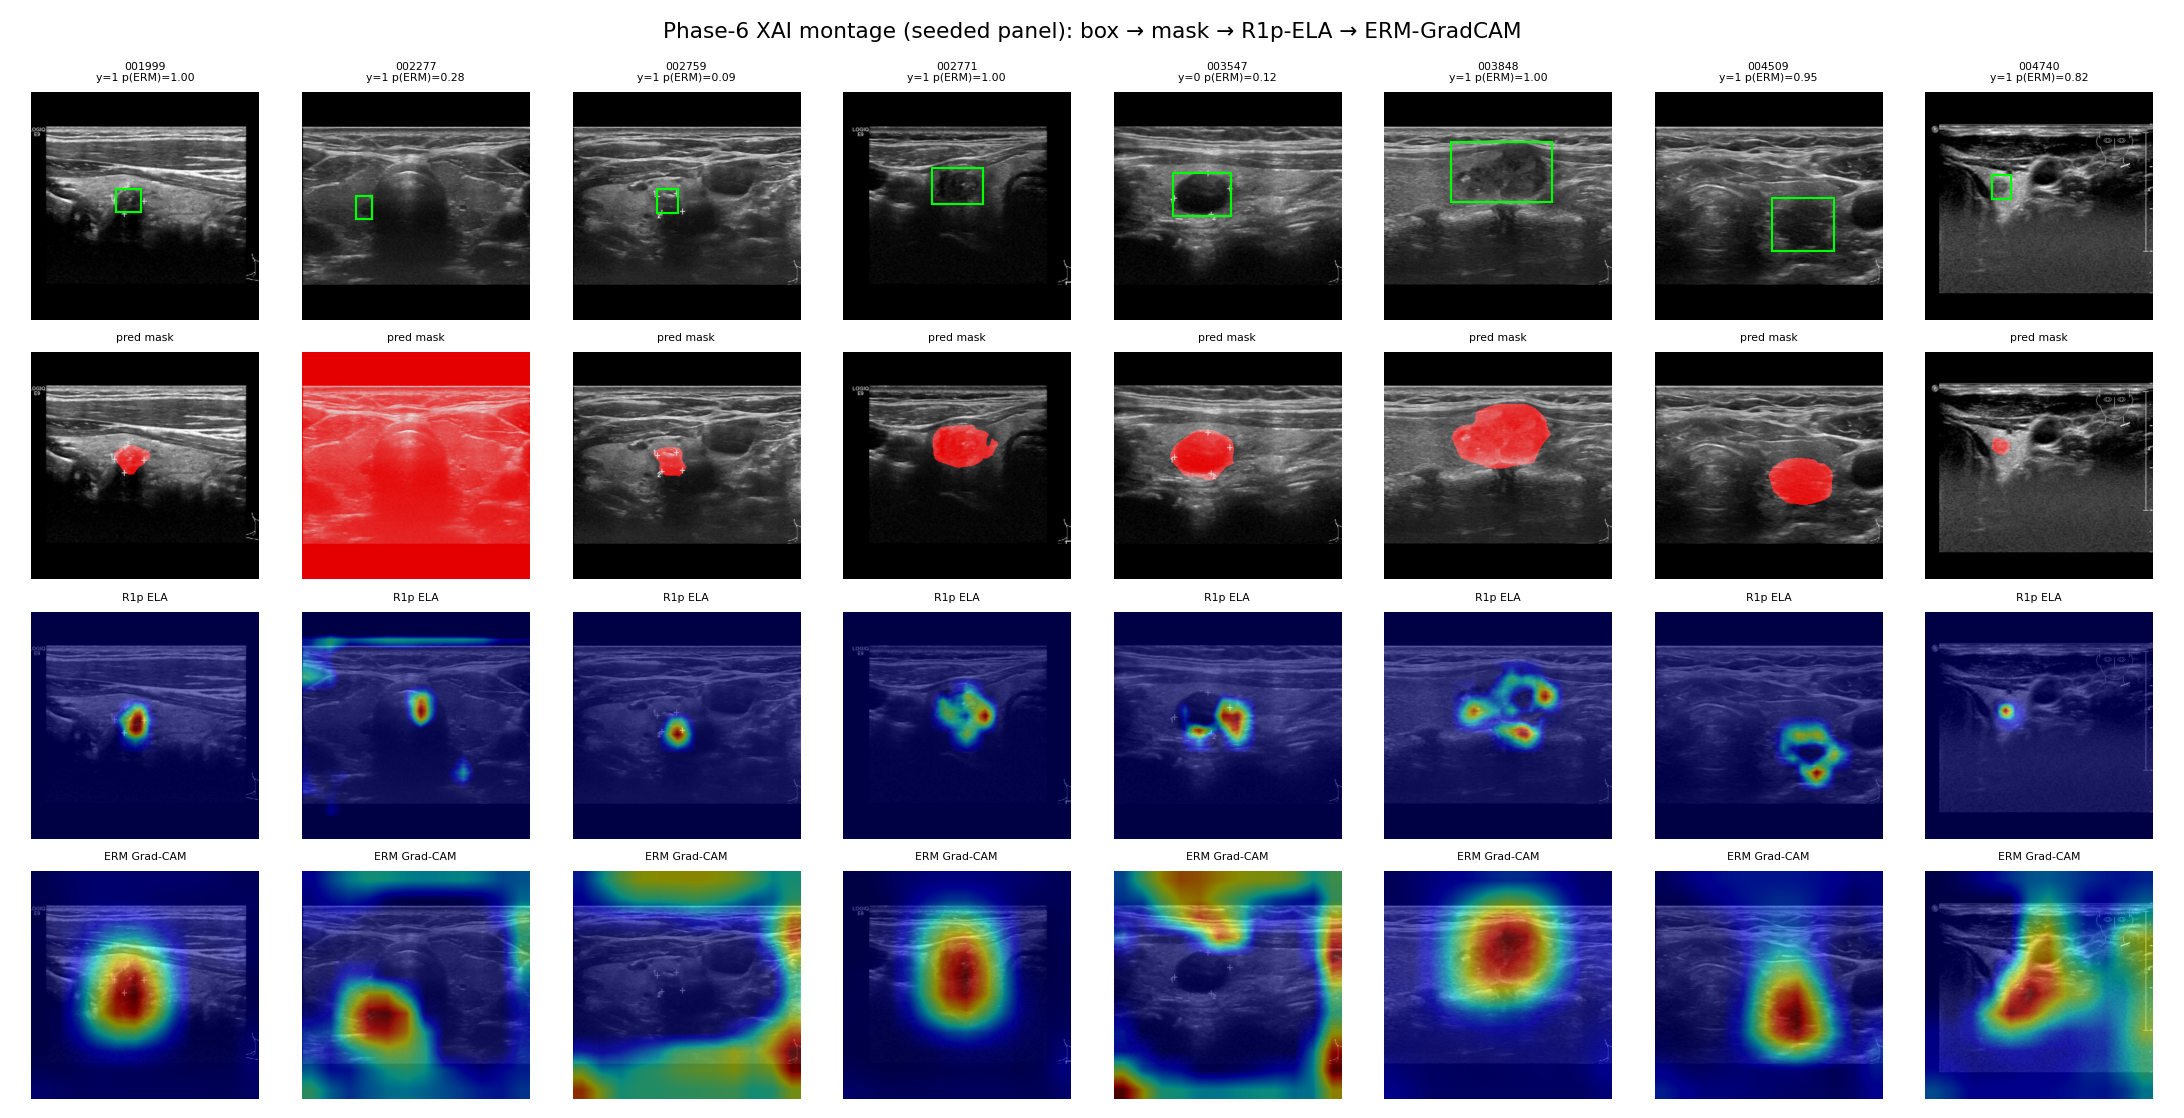
\includegraphics[width=0.98\linewidth]{phase6_cam_montage.png}
\caption{\textbf{Lesion-grounded explanations on representative cases.}
Rows: TN5000-test and ThyUS-600 cases (labels given). Columns: raw
B-mode frame with expert box; frozen predicted mask; R1p-ELA; Grad-CAM
(with the model's probability). The grounded attribution is confined to
the nodule by construction; Grad-CAM energy disperses into gland tissue
and acquisition artefacts, visibly more so on the external rows.}
\label{fig:montage}
\end{figure}

\begin{figure}[H]
\centering
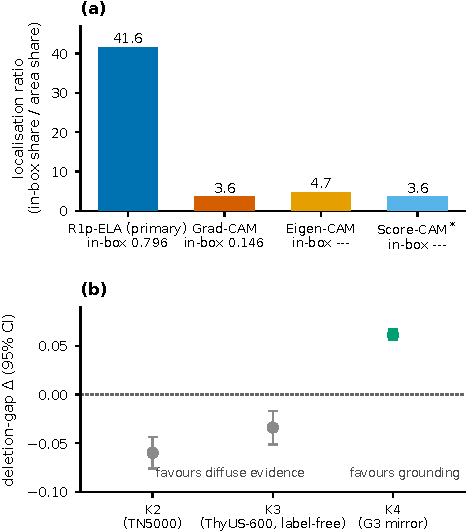
\includegraphics[width=0.95\linewidth]{fig5_explainability.pdf}
\caption{\textbf{Explanation quality by axis (Phase 6, family K).}
(a) Localisation against TN5000 expert boxes: R1p-ELA concentrates an
order of magnitude more of its mass on the nodule than Grad-CAM,
Eigen-CAM, or Score-CAM (paired $\Delta$ K1 $=+38.0$, CI
35.35..40.83, $p{<}0.0004$); in-box share printed per bar ($^*$Score-CAM
on the seeded $n{=}150$ subsample). (b) Deletion-gap deltas show the
complementary, metric-driven face: K2/K3 are significantly negative
(removal-based faithfulness rewards diffuse evidence; mechanism in
text), while within the joint pair the grounded head wins as the
mechanism predicts (K4). CIs: 5{,}000-resample paired bootstrap;
Bonferroni $\alpha{=}0.0125$.}
\label{fig:explainability}
\end{figure}


The battery ran unmodified on TN5000-test ($n{=}950$, 693 malignant,
expert boxes on all 950 images) and the seeded ThyUS-600 first-image
panel ($n{=}600$, 376 malignant; drawn from the licensed 839-case
cohort and triangulated: 522 malignant, 8{,}465 images, prevalence
0.6222). Integrity structure held end-to-end: live probabilities
reproduce the Phase-3/4 archives (ERM 0.9404 vs 0.9401; R1p 0.8889 vs
0.8889; JOINT arms to ${\leq}2.25{\times}10^{-5}$ max $|\Delta p|$
against the $10^{-4}$ gate), and the 32-image ELA exactness probe
confirmed the closed-form logit decomposition (max deviation
R0 $1.6{\times}10^{-6}$, R1p $2.9{\times}10^{-7}$, R2p
$2.7{\times}10^{-7}$, JOINT-g $7.8{\times}10^{-8}$, JOINT-img
$2.6{\times}10^{-8}$; gate $10^{-3}$). All inferential
statements use 5{,}000 paired image-level resamples at Bonferroni
$\alpha{=}0.0125$ (seed 42); empirical $p{=}0.0$ is typeset
$p{<}0.0004$. A seeded qualitative panel accompanies the quantitative
tests (Fig.~\ref{fig:montage}).

The primary test is decisive (Table~\ref{tab:phase6_familyk};
Fig.~\ref{fig:explainability}; per-map statistics: Supplementary
Table~S18). Against expert-annotated nodule boxes, R1p-ELA attains a
localisation ratio of 41.6 (median 27.8) where Grad-CAM attains 3.6: a
paired separation of K1 $\Delta = +38.00$ (95\% CI 35.35..40.83,
$p{<}0.0004$). The gap is not an artefact of the comparator: Eigen-CAM
and Score-CAM sit at 4.7 and 3.6, an order of magnitude below the
grounded explanation. The decomposition marks R1p's precision as
segmenter-grade (79.6\% of attribution mass inside the box, normalised
entropy 0.717) against ERM-family diffusion (in-box mass 0.146,
entropy 0.928). The pointing game cuts the other way descriptively
(Eigen-CAM 0.736 $>$ R1p 0.637 $>$ Score-CAM 0.580 $>$ Grad-CAM 0.514):
where a diffuse map happens to peak inside the box it scores like a
concentrated one; the ratio and in-box-mass statistics instead report
where the \emph{bulk} of the explanation lies. Under shift, ERM's
attention deserts the nodule: Grad-CAM's energy inside the frozen
predicted mask falls from 0.1253 in-domain (${\approx}3.2\times$ the
mask's area share) to 0.0549 on ThyUS-600 (${\approx}1.3\times$).

The faithfulness pair is honestly null-to-reversed for the intended
direction, and we report it as such (K2: $-0.0598$, CI
$-0.0761..-0.0437$, $p{<}0.0004$ on TN5000; K3: $-0.0339$, CI
$-0.0511..-0.0171$, $p{<}0.0004$ as the label-free external
replication; rows: Supplementary Table~S22). Inspection shows the
reversal is carried by the random-order control, not by the guided
curves: explanation-guided deletion degrades
both models essentially identically (areas 0.3334 vs 0.3315), while
random deletion erodes the diffuse image-wide classifier more slowly
(random-control areas 0.4986 vs 0.5564; deletion/insertion areas:
Supplementary Table~S19). The deletion-gap statistic rewards redundant, spatially spread evidence
rather than explanation quality per se --- the known sensitivity of
removal-based metrics to the model's evidence distribution.
Insertion (descriptive, $n{=}300$) favours ERM (0.2043 vs 0.0351) with
the same proviso, compounded by the out-of-distribution nature of
sharp-lesion-on-blur hybrids for a mask-conditioned head. Within the
joint pair, however, grounding helps exactly as the G3 mechanism
predicts (K4: $+0.0613$, CI 0.0560..0.0667; Supplementary Table~S22),
the deletion-gap ladder rising monotonically with the degree of
built-in grounding (JOINT-img 0.041 $<$ JOINT-g 0.102 $<$ R1p 0.165).

Stability is mixed and instructive (Supplementary Table~S20): under
intensity noise R1p-ELA is the more stable explanation in both domains
(mean Spearman 0.921 vs 0.832 on TN5000; 0.799 vs 0.755 on ThyUS-600),
while affine warps invert the ordering (0.771 vs 0.871; 0.640 vs
0.810) --- the two rows are the same concentration geometry read in
opposite directions; concentrated maps are penalised by per-pixel
correlation after geometric displacement, additive noise taxing
diffuse maps more. These axes were pre-declared non-gated and are
reported descriptively.

The randomisation cascade produced the battery's one failed gate, and
we report it as such (Supplementary Table~S21). R1p, whose design
admits only a head-level stage (the frozen trunk is the shared
measurement instrument), retains mean $|\rho|{=}$ 0.2991 --- the gate
fails against the pre-registered $|\rho|{<}0.2$ bar. ERM decorrelates
below the bar only at its deepest stage (0.1205), and at the matching
shallow stage (fc only, 0.2948) it fails identically: a 0.2 threshold
at readout depth is unattainable for either model, rather than evidence
of explanation defect. Two follow-up diagnostics, whose decision rules
were committed before they were run, localise the result. Independent
resampled heads correlate at only 0.0920 on the same images, so the
retained 0.2991 sits $+0.2072$ above that floor: the pixel map is
\emph{not} head-agnostic geometry. Meanwhile, the per-feature logit
attribution decorrelates completely under head resampling (Spearman
$-0.0150$, $|{-}|$ 0.0191; Pearson $-0.0016$). Combined with the exactness gate, the operational picture
is precise: the ELA attribution is the exact, weight-specific
decomposition of the linear head in feature space, and its pixel-space
rendering is partly bound by the shared in-lesion feature field ---
which is precisely the lesion grounding the architecture exists to
provide, and which K1 shows is where the explanation correctly lives.

\begin{table}[!ht]
\centering\scriptsize
\caption{Phase-6 pre-registered family K (image-level paired bootstrap,
5{,}000 resamples, seed 42; Bonferroni $\alpha{=}0.0125$; two-sided
empirical $p$, with $p{=}0.0$ typeset $p{<}0.0004$; point estimates are
bootstrap-distribution means --- for the heavy-tailed K1 ratio the mean
of replicate means (38.0047) deviates from the arithmetic mean of
differences (38.0270) by 0.0223, ${\approx}1.1\times$ the Monte-Carlo
standard error, as expected). K3 is label-free and therefore independent
of the Phase-5 licence. Significance column: Bonferroni verdict.}
\label{tab:phase6_familyk}
\begin{tabular}{llllccl}
\toprule
Test & Metric & A & B & $\Delta$(A$-$B) (95\% CI) & Sig. & Note \\
\midrule
K1 & localisation ratio & R1p-ELA & ERM-GradCAM & $+38.0047$ (35.3461..40.8339) & YES & PRIMARY plausibility \\
\bottomrule
\end{tabular}

{\footnotesize Secondary contrasts K2--K4, relocated row-for-row: Supplementary Table~S22.}
\end{table}

% Phase 7 (edge-feasibility simulation) descoped 2026-08-23 by operator
% decision; methodology retains only a labelled future-work outlook.

% ======================================================================
% sec16_discussion.tex — 16-page Discussion + Limitations/Future + Conclusion
% Compressed 2026-08-23 from discussion_conclusion_draft.tex (2,610w ->
% ~1,750w). Verdict-first structure retained; every number survives
% verbatim (token-gate verified vs orig union); all nine hypotheses carry an
% explicit verdict. SM pointers are textual (SM docs are separate).
% ======================================================================
\section{Discussion}\label{sec:discussion}

This study asked whether few-shot, support-conditioned nodule segmentation
can improve cross-domain thyroid-ultrasound malignancy classification while
providing calibrated, anatomically grounded, and faithful explanations
(Section~\ref{sec:research_questions}). The answer across six executed and
locked phases is deliberately three-part. \emph{Anatomical grounding: yes,
decisively} --- the grounded explanation is an order of magnitude more
lesion-aligned than any unconstrained-CAM comparator, and the grounded
operating point replicates on an independent pathology-confirmed case-level
cohort with an eleven-fold sensitivity advantage over the fine-tuned
classifier. \emph{Calibration: no} --- no model's calibration survives
prevalence shift, and we report this rather than recalibrating on target
data. \emph{Faithful: yes in feature space, reversed on removal-based
metrics} --- and the reversal itself carries a methodological lesson about
what deletion-style statistics measure.

\paragraph{Few-shot segmentation and annotation efficiency (RQ1, RQ2; H1,
H2).}
Few-shot support conditioning delivers near-ceiling nodule segmentation
with almost no annotation, in-domain and zero-shot. A learned fusion
decoder beats parameter-free prototype matching in all 20
condition--budget cells ($+3.2$ to $+20.9$ Dice points at $K{=}20$); the
parameter-free variant collapses to 0.47--0.57 Dice under zero-shot
transfer, so the contribution sits in the decoder, not in nearest-prototype
matching of the PANet kind~\cite{rev_wang2019panet,rev_tian2020pfenet,rev_min2021hsnet}.
The budget saturates early: $K{=}5$ nested support masks already deliver
98.6--99.5\% of the $K{=}20$ score in every condition
(Table~\ref{tab:phase2}), a direct quantification of dense-label
efficiency (Gap~1); and zero-shot transfer with \emph{source} supports
lands within 3.9 (TNUI-2021) and 6.1 (DDTI) Dice points of the fully
supervised external reference at zero target annotation (Supplementary
Table~S2)~\cite{rev_gong2021tn3k,rev_pedraza2015ddti}.
H1 (annotation efficiency) is therefore \emph{supported}, and in a
stronger form than posed: the support mechanism substitutes for target
annotation entirely. H2 is \emph{not supported in its strong form}: the
few-shot model narrows but does not eliminate the supervised external
gap. Two honest qualifications apply. The support-domain bias on TNUI
--- target supports underperform source supports (0.6804 vs 0.7079 at
$K{=}20$) --- inverts the intuition that target-side support always
helps; we report it as a limitation rather than tune it away. DDTI is
the hardest masked cohort for both paradigms (supervised 0.7396;
zero-shot 0.6782), consistent with its doubled boundary error (median
HD95 ${\approx}22$ vs 10--11 px) and burned-in annotations.

\paragraph{Does grounding improve classification? (RQ3, RQ6; H3, H6).}
Grounding improves the frozen operating point substantially, cohort-wide
ranking not at all, and calibration never. In-domain on
TN5000-test~\cite{rev_zhang2025tn5000}, the grounded linear head beats the
identical whole-image head (T1: $+0.0368$ AUROC, $p{=}0.0004$), and the
grounded label-budget curve dominates the image budget at every support
size, saturating by 50 labels per class and staying within 0.013--0.029 of
the ground-truth-box oracle (Supplementary Table~S8). The fine-tuned ERM
remains the in-domain rank and operating-point ceiling (T2, T5) --- a fact
we retain rather than minimise, because the external phases invert it: At the frozen specificity-0.90 operating point the
grounded head's advantage replicates across the TNUI institutional family
(pooled P5: $+0.120$ sensitivity over ERM, $p{<}0.0004$; third cohort F5:
$+0.126$, $p{<}0.0004$), reverses on the independent DDTI cohort (E5:
$-0.146$, $p{=}0.0012$; burned-in annotations documented), and replicates
again --- at case level, against a pathology gold standard, on 839
ThyUS2Path~\cite{rev_hou2024thyus2path} cases untouched by any tuning ---
with J1 $+0.1457$ ($p{<}0.0004$; McNemar 77 vs 1). \emph{Rank}
discrimination does not travel: external AUROCs are cohort-dominated (even
true-mask oracles span 0.41--0.85), and on ThyUS2Path every model
collapses to 0.478--0.548 with AUPRC at the 0.622 prevalence floor. H3 is
thus \emph{supported for the operating point, null for ranking, and
refuted for calibration}: the grounding signal concentrates at the frozen
operating point --- the quantity fixed before external data were seen ---
while ranking is dominated by site-specific case-mix structure no frozen
rule escaped (Table~\ref{tab:evidence}; cf.~retrospective multi-cohort
thyroid CAD~\cite{rev_li2019multicohort}). RQ6 receives a clean null: the
peri-lesional context ring adds nothing (T4: $+0.0074$, $p{=}0.139$),
replicating across the prototype sweep at every budget under a different
head family. H6 is \emph{refuted}, twice --- constraining the ROI+context
premise for nodule classification~\cite{rev_yavuz2026roicontext}: on
frozen descriptors, context contributes neither discrimination nor label
efficiency; it merely dilutes what is already lesion-local.

\paragraph{Error propagation (RQ4; H4).}
Replacing expert boxes with predicted masks costs a small, bounded, and
diffuse tax, and no confidence gate can waive it. T3 prices the
replacement at ${\approx}2$ AUROC points ($+0.0202$, $p{=}0.0048$) and T6
at ${\approx}10$ operating-point points. Crucially the tax is
\emph{diffuse}, not catastrophic: stratified by predicted-mask confidence,
the oracle-minus-predicted gap does not localise to bad segmentations and
is descriptively largest in the \emph{highest}-confidence quartile
(Supplementary Table~S7). H4's first clause (a small, budget-shrinkable
gap) is supported; its second (uncertainty identifies the worst cases) is
\emph{not}. For a pipeline claim this is the useful form: predicted-mask
classification deploys end-to-end at a known, bounded cost, and mask
confidence should not be used to waive caution.

\paragraph{Partial supervision and the joint dilemma (RQ5; H5).}
An intact segmenter and the fine-tuning premium cannot be had at once:
the dilemma, not either protocol, is the finding. The naive joint
fine-tune failed its own pre-registered non-collapse gate (Dice 0.669
against a gate of 0.797); the corrected protocol (frozen-head warmup,
$10^{-5}$ joint phase, seg-guarded selection) preserved the segmenter and
passed both gates. The intact segmenter is \emph{then} what sacrifices the
fine-tuning premium: the T2 gap widened (G1 $-0.0703$),
the joint model sat below its frozen counterpart (G2 $-0.0205$), lost
outright at the frozen operating point (G4; McNemar 41 vs 206), and
transferred externally worse than the frozen grounded head (H2
$-0.0534$). Yet under identical joint conditions, grounding beat
multi-tasking by $+0.1489$ AUROC (G3;
Table~\ref{tab:phase4_families}): the grounding, not the freezing,
carries the signal. H5 is \emph{refuted in this instantiation}, and the
refutation is informative: closing the fine-tuning gap requires exactly
the representational reorganisation that a segmentation non-collapse
constraint forbids.

\paragraph{Uncertainty, calibration, and referral (RQ7; H7).}
Calibration never survives the shift, but confidence-based referral still
removes most of the frozen operating point's malignant misses. External
ECE sits at 0.25--0.42 for every head after prevalence shift; on
ThyUS2Path five of six models deteriorate \emph{further} after
source-fitted temperature scaling, so deployment-level use requires local
recalibration. What does work, with nothing refitted, is selective
prediction on the calibrated margin: retaining the most-confident 70\%
lifts in-domain sensitivity at spec90 from 0.564 to 0.840, with the
external pool tracking closely (Supplementary Table~S14); at 50\%
coverage, external sensitivity reaches 0.897. The mechanism is
referral-shaped --- 86--87\% of the malignant cases missed at the frozen
point sit inside the abstained lower-confidence half on both panels ---
so abstention selectively clears threshold-proximal malignancies rather
than globally inflating accuracy. H7 is \emph{supported}: a small
referral stream (${\approx}30$\% of cases) removes the majority of the
frozen point's false negatives without touching a single parameter.

\paragraph{Explanation reliability (RQ8; H8).}
The pre-registered battery (family K) gives H8 a split verdict by clause,
and we regard the split as a methodological contribution.
\emph{Lesion overlap: decisive support.} Against expert boxes, the
grounded, exact linear attribution attains a localisation ratio of 41.6
against 3.6 for Grad-CAM~\cite{rev_selvaraju2017} (K1 $+38.0$, CI
35.35..40.83, $p{<}0.0004$), with Eigen-CAM and Score-CAM
controls~\cite{rev_muhammad2020eigencam,rev_wang2020scorecam} at 4.7 and
3.6 --- the separation is a property of grounding, not of Grad-CAM's
weakness. The descriptives cohere: 79.6\% of the grounded map's mass lies
inside the expert box versus 14.6\% for Grad-CAM, whose agreement with the
predicted nodule falls from ${\approx}3.2\times$ area share in-domain to
${\approx}1.3\times$ on ThyUS-600: under shift, the fine-tuned
classifier's attention deserts the lesion; the grounded mechanism's
definitionally cannot. \emph{Perturbation stability: partial support} ---
the grounded map is the more stable under intensity noise in both domains,
the less stable under affine warps (Supplementary Table~S20), the
expected signature of concentrated versus diffuse maps.
\emph{Deletion/insertion faithfulness: not supported as posed.} K2 and K3
are significant in reverse ($-0.0598$, $-0.0339$), with identical
explanations under guidance but divergent random-ordering controls:
removal-based faithfulness here rewards redundant, spatially spread
evidence rather than explanation fidelity, the documented sensitivity of
this metric family to evidence
distribution~\cite{rev_samek2017,rev_hooker2019,rev_petsiuk2018rise}.
Inside the joint pair, where the confound cancels, grounding wins exactly
as the mechanism predicts (K4 $+0.0613$). The randomisation cascade adds
the final honest note: the readout-level R1p cascade fails its gate
(0.2991 against the 0.2 bar --- which the ERM readout-only stage, 0.2948,
fails equally); committed diagnostics show the retention is neither
head-agnostic geometry (random-vs-random floor 0.092; retained elevation
$+0.2072$ above it) nor a broken explanation (per-feature attribution
decorrelates completely, $\rho=-0.015$; exactness
${\le}1.6{\times}10^{-6}$). H8 is therefore
\emph{supported on overlap, partially on stability, and refuted as stated
on removal-based faithfulness} --- the hypothesis's conjunction, rather
than the pipeline, is what the measurements reject. The take-away is to
pre-register plausibility and faithfulness separately and interpret each
against its explanation's geometry~\cite{rev_adebayo2018}; a pooled
``trustworthy CAM'' claim, of the kind thyroid CAD papers routinely
display only
qualitatively~\cite{rev_yao2023tinet,rev_song2023explainer,rev_nguyen2023trust,rev_ahmed2026xai},
would obscure exactly that split.

\paragraph{Cross-cutting interpretation.}
Three themes unify the six phases. \emph{First, the operating point is the
unit of transfer}: every robust external result lives at thresholds frozen
before external data were touched (P5, F5, J1); every cohort-wide rank
comparison yields cohort-dominated heterogeneity instead --- post-hoc
threshold selection would have written a different, irreproducible paper.
\emph{Second, the external-validity gradient is informative, not
embarrassing}: transfer holds within the TNUI family, inverts on DDTI
under a documented annotation confound, and re-emerges on ThyUS2Path at
case level against the strongest label standard; a single pooled external
AUROC would have concealed all of that. \emph{Third, pre-registered gates
are content, not ceremony}: the failed gates --- the joint protocol's
segmentation collapse (v1), the cascade's R1p stage, the DDTI
counterexample, H6's double null --- shaped the model choice (frozen R1p
as primary), the XAI interpretation, and the scope of the claims. This is
the reproducibility practice Gap~8 calls for, applied to our own pipeline
first.

\paragraph{Limitations and future work.}
Several limitations bound the claims. (i) External \emph{absolute}
performance on ThyUS2Path is far from diagnostic grade for every model
(15.9\% sensitivity at 90\% specificity for the best head); the cohort is
a stress test of what survives shift, and all external comparisons are
relative statements at frozen operating points. (ii) The zero-shot
empty-mask fallback rate on ThyUS2Path runs at 10.9\% of images (22\% of
case-first images), so a nontrivial external minority is scored by the
whole-image fallback pathway. (iii) TNUI-2021 benign counts are small (5
test, 16 validation), limiting cohort-level precision, and DDTI carries
burned-in acquisition annotations as a documented confound. (iv) K1
evaluates against boxes rather than pixel masks, so the localisation
reward is at box granularity; and the qualitative evidence is a montage,
not a reader study --- human-usefulness evaluation with clinicians
remains open. (v) The frozen-descriptor heads are confidence-under-scaled
in-domain ($T{<}1$) and all models require local recalibration before any
deployment interpretation. (vi) Phase 1's reference is single-seed, and
the joint model had not saturated at its pre-registered epoch cap, making
family-G magnitudes conservative. (vii) The cascade gate failure means
pixel-space attribution maps should be read as partly bound to the
in-lesion feature field even though their feature-space decomposition is
exact and weight-specific; we have bounded, not eliminated, that
ambiguity. The natural next experiments follow directly: the descoped
edge-feasibility pathway (RQ9/H9) admits a gradient-free deployment mode
with cached prototype vectors, to be benchmarked as an offline simulation
rather than a clinical device; mask-uncertainty estimators that
\emph{do} localise classification risk (the present confidence quartiles
do not); and a prospective multi-institution evaluation with per-site
calibration, which the audit-gated protocol is designed to absorb without
modification.

\paragraph{}\noindent In conclusion, we present a lesion-grounded,
prototype-based few-shot framework
(LG-PM) for annotation-efficient thyroid-ultrasound diagnosis, evaluated
across a fully pre-registered, audit-trailed programme. The central
question receives a disciplined answer. Support-conditioned segmentation
transfers nodule localisation to unseen ultrasound domains with zero
target annotation, coming within a few Dice points of the fully
supervised external reference and saturating after a handful of support
masks. The predicted masks feed a classification pathway whose advantage
is real and specific: lesion grounding beats identical whole-image heads
in-domain, and --- uniquely in this study --- its operating-point
advantage replicates externally, culminating in an eleven-fold case-level
sensitivity advantage over fine-tuned classification on the
pathology-confirmed ThyUS2Path cohort. That advantage does not extend to
cohort-wide ranking, calibration, or removal-based faithfulness, each of
which we report as measured: rank transfer collapses under shift for all
models including oracles, calibration requires local refit, deletion-style
metrics reward diffuse-evidence models, and one randomisation gate failed
and is reported as failed. The framework does not diagnose cancer, and its
external ranking and calibration limits are the honest boundary of the
claim. What it establishes is that in thyroid ultrasound, lesion grounding
is a transferable operating-point advantage with anatomically aligned,
exact, and audit-trailed explanations --- delivered at a fraction of the
annotation cost of supervised adaptation.


\supplementary{The supplementary material is available online, comprising Tables S1--S22 and Figures S1--S2 referenced throughout the Results, plus extended methodological detail, a reproducibility artefact manifest, and an algorithmic summary (Algorithm S1).}

\conflictsofinterest{The authors declare no competing interests.}

\funding{The authors received no specific funding for this work.}

\availabilityofdataandmaterials{All datasets are publicly available from their original publications (cited in the text). No new imaging data were generated.}

\backnotes{Code Availability}{Notebooks, seeds and audit artefacts for every phase are archived in the project ledger. Code is available from the corresponding author upon reasonable request.}

\ethicsapproval{All cohorts analysed are public, de-identified datasets (TN3K/TN5000, TNUI-2021, DDTI, ThyUS2Path); no new human data were collected. Ethics approval was not required for this secondary analysis.}

\acknowledgement{Not applicable.}

\authorcontributions{All authors contributed to the study conception and design. Material preparation, data collection, and analysis were performed collaboratively. All authors read and approved the final manuscript.}


\reftitle{References}
\bibliography{references}

\end{document}
